% -------------------------------
% CIDaeN: Plantilla para la elaboración del TFM. Versión 0.0 
%
% Luis de la Ossa. UCLM
% 
% Compilar con XeLaTeX 
% -------------------------------
\documentclass[12pt, a4paper]{book}

% -------------------------------
% Información y opciones del documento. Debe editarse.
% -------------------------------
% -------------------------------
% CIDaeN: Plantilla para la elaboración del TFM. Versión 0.0 
%
% Luis de la Ossa. UCLM
% 
% Compilar con XeLaTeX 
% -------------------------------


% -------------------------------
% Comandos comunes
% -------------------------------
\newcommand{\uclm}{Universidad de Castilla-La Mancha\,}
\newcommand{\dsi}{Departamento de Sistemas Informáticos\,}
\newcommand{\esii}{Escuela Superior de Ingeniería Informática de Albacete\,}



% -------------------------------
% Comandos específicos
% -------------------------------
\newcommand{\autor}{Luna Jiménez Fernández\,}
\newcommand{\titulo}{WiDS Datathon 2024 - Challenge 2:\\
	Modelos de regresión para estimación del periodo de diagnóstico metastático\,}
\newcommand{\director}{Juan Carlos Alfaro Jiménez\,}
\newcommand{\codirector}{\,}
\newcommand{\fecha}{Junio, 2025\,}








% -------------------------------
% Configuración del documento, paquetes, etc. 
% -------------------------------
% -------------------------------
% CIDaeN: Plantilla para la elaboración del TFM. Versión 0.0 
%
% Luis de la Ossa. UCLM
% 
% Compilar con XeLaTeX 
% -------------------------------


% -------------------------------
% Idioma
% -------------------------------
\usepackage{polyglossia}
\setmainlanguage{spanish}


% -------------------------------
% Fuente
% -------------------------------
% Cualquier tamaño de texto: {\fontsize{100pt}{120pt}\selectfont tutexto}
\usepackage{anyfontsize}
% Selección de fuentes.
\usepackage{fontspec}
% Espacio entre líneas
\usepackage{setspace}
% Fuentes especiales
\usepackage{textcomp,marvosym,pifont}


% -------------------------------
% Otros paquetes de uso común
% -------------------------------
% Símbolos matemáticos
\usepackage{amsmath,amsfonts,amssymb}
% Gráficos
\usepackage{graphicx}
% Posición arbitraria de los gráficos
\usepackage[absolute,overlay]{textpos}
% Apéndices
\usepackage{appendix}


% -------------------------------
% Esquema de colores
% -------------------------------
% Paquete para la definición de colores
\usepackage[table]{xcolor}
% Esquema de colores
% -------------------------------
% Plantilla del TFG en la ESIIAB-UCLM. Versión 0.0 (Preliminar)
%
% Luis de la Ossa
% 
% Compilar con XeLaTeX 
% -------------------------------


% -------------------------------
% Esquema de colores
% -------------------------------
% Estos balores coinciden con colores de OpenOffice 
% Se pueden redefinir para que coincidan con las paletas de las 
% herramientas utilizadas para hacer las gráficas.
\definecolor{blanco}{RGB}{255,255,255} 
\definecolor{negro}{RGB}{0,0,0}
\definecolor{gris95}{gray}{.95}
\definecolor{gris75}{gray}{.75}
\definecolor{gris50}{gray}{.50}
\definecolor{gris25}{gray}{.25}
\definecolor{rojo}{RGB}{172,39,0}        
\definecolor{azul}{RGB}{2,87,108}        
\definecolor{verde}{RGB}{0,116,70}     
\definecolor{naranja}{RGB}{224, 119, 20} 
\definecolor{mostaza}{RGB}{226, 182, 21} 

% Negrita con color definido 
\newcommand{\bfa}[1]{\textcolor{azul}{\bf #1}} 
\newcommand{\bfr}[1]{\textcolor{rojo}{\bf #1}}
\newcommand{\bfn}[1]{\textcolor{naranja}{\bf #1}}
\newcommand{\bfv}[1]{\textcolor{verde}{\bf #1}}  
\newcommand{\bfm}[1]{\textcolor{mostaza}{\bf #1}} 



% -------------------------------
% Color del tema
% -------------------------------

% Color para los títulos, etc.
%\definecolor{tema}{RGB}{0,0,0}        % Negro 
\definecolor{tema}{RGB}{2,87,108}      % Azul del esquema  

% Negritas con el color del tema
\newcommand{\bft}[1]{\textcolor{tema}{\bf #1}} 



% -------------------------------
% Márgenes
% -------------------------------
% Márgenes de las páginas
\usepackage[
  inner	 =	3cm,   % Margen interior
  outer	 =	2.5cm, % Margen exterior
  top	 =	2.5cm, % Margen superior
  bottom =	2.5cm, % Margen inferior
  includeheadfoot, % Incluye cabecera y pie de página en los márgenes
]{geometry}
% Muestra una regla para comprobar el formato de las páginas (descomentar)
%\usepackage[type=upperleft,showframe,marklength=8mm]{fgruler} 


% -------------------------------
% Renombra tablas y bibliografía
% -------------------------------
\addto\captionsspanish{
	\renewcommand{\listtablename}{Índice de tablas} 
	\renewcommand{\tablename}{Tabla}
	\renewcommand{\bibname}{Referencia bibliográfica}
}


% -------------------------------
% Itemize y enumerate. Control de los espacios.
% -------------------------------
\usepackage{enumitem}
\setitemize{itemsep=0pt}
\setenumerate{itemsep=0pt}
\renewcommand{\labelitemi}{\tiny\bft{$\blacksquare$}}
\renewcommand{\labelitemii}{\bft{$\bullet$}}
\renewcommand{\labelitemiii}{\bft{-}}


% -------------------------------
% Enlaces y colores
% -------------------------------
\usepackage[hidelinks]{hyperref}
%\hypersetup{
%    colorlinks,
%    citecolor=black,
%    filecolor=black,
%    linkcolor=black,
%    urlcolor=black
%}

% -------------------------------
% Gestión de elementos flotantes
% -------------------------------
% Para forzar a que las figuras aparezcan antes del fin de una sección.
%\usepackage[section]{placeins}

% Gestión de títulos de los elementos flotantes
\usepackage{caption}
% Subfiguras y títulos en subfiguras
\usepackage{subcaption}

% Títulos
\DeclareCaptionFont{tema}{\color{tema}} % Color
\captionsetup{labelfont={tema, bf}}     % Estilo
\captionsetup{font=normalsize}          % Tamaño
\captionsetup{width=.9\linewidth}       % Anchura del título
 % Distancia de la figura al texto.
\setlength{\intextsep}{1cm} 
\setlength{\textfloatsep}{1cm}         
       

% -------------------------------
% Utilidades para tablas
% -------------------------------
% Para fundir filas en tablas
\usepackage{multirow}
% Para definir columnas con ancho fijo y alineación
\usepackage{array,ragged2e}
\newcolumntype{L}[1]{>{\raggedright\let\newline\\\arraybackslash\hspace{0pt}}m{#1}}
\newcolumntype{C}[1]{>{\centering\let\newline\\\arraybackslash\hspace{0pt}}m{#1}}
\newcolumntype{R}[1]{>{\raggedleft\let\newline\\\arraybackslash\hspace{0pt}}m{#1}}


% -------------------------------
% Para tabular
% -------------------------------
\usepackage{tabto}


% -------------------------------
% Formato de títulos, capítulos, etc.
% -------------------------------
\usepackage{titlesec, titletoc}
% Parte
\titleformat{\part}[display]												   	   % Estilo
	{\Huge \centering \color{tema}}                                                % Formato
	{Parte \thepart }                                                              % Etiqueta
	{0.75ex}                                                                       % Separación
	{\bfseries\fontsize{25pt}{40pt}\selectfont}                                    % Entre etiqueta y título            
	[\thispagestyle{empty}]                                                        % Después

% Capítulo		
\titleformat{\chapter}[block]            			 			                    % Estilo  	
	{\vspace{0cm} \flushright \bfseries \LARGE \color{tema}}  	        			% Formato 
	{\thechapter.}                  			  									% Etiqueta
	{0.75ex}                                     									% Separación
	{}                                           									% Entre etiqueta y título
	[\vspace{0.1cm} \rule{0.5\textwidth}{1pt}\vspace*{1cm}\thispagestyle{plain}]    % Después      
  
% Sección
\titleformat{\section}
	{\vspace{5pt}  \Large \color{tema}}
	{\thesection .}
	{0.75ex}
	{}

% Subsección
\titleformat{\subsection}
	{\large \color{tema}}
	{\thesubsection .}
	{0.75ex}
	{}
 
% Subsubsección
\titleformat{\subsubsection}
	{\bf\color{tema}}
	{}
	{0.75ex}
	{}
	 
% Parte (TOC)
\titlecontents{part}[2pc]
  	{\vspace{20pt}\bfseries\filright\Large\color{tema}}
  	{\contentslabel{1.5pc}}{\hspace*{-1.5pc}}
  	{\vspace{5pt}}
  	{}
  
% Capítulo (TOC)
\titlecontents{chapter}[2pc]
  	{\vspace{10pt}\bfseries\large\filright}
  	{\contentslabel{1.5pc}}{\hspace*{-1.5pc}}
  	{\mdseries\titlerule*[0.5pc]{.}\bfseries\contentspage}

% Sección (TOC)
\titlecontents{section}[4pc]
  	{\vspace{5pt}\filright}
  	{\contentslabel{2pc}}{\hspace*{2pc}}
  	{\titlerule*[0.5pc]{.}\contentspage}
  	{\vspace{5pt}

% Subsección (TOC)
\titlecontents{subsection}[6pc]
  	{\vspace{2.5pt}\filright\small\em}
  	{\contentslabel{3pc}}{\hspace*{-3pc}}
  	{\titlerule*[0.5pc]{.}\contentspage} 
  	
  	
% -------------------------------
% Cabeceras y pie de página
% -------------------------------
\usepackage{fancyhdr}
\pagestyle{fancy}
\fancyhf{}

% Permite incluir la parte. Para ello crea \parttitle
\let\Oldpart\part
\newcommand{\parttitle}{}
\renewcommand{\part}[1]{\Oldpart{#1}\renewcommand{\parttitle}{#1}}

% Cabeceras y pies de página
\fancyhead[LE]{}
\fancyhead[RO]{\slshape \leftmark}
\fancyfoot[LE,RO]{\thepage}
\renewcommand{\footrulewidth}{1pt}
\renewcommand{\headrulewidth}{1pt}
\renewcommand{\chaptermark}[1]{\markboth{#1}{}} % Capítulo (Solo texto)
\renewcommand{\chaptermark}[1]{\markboth{\thechapter. #1}{}} % Capítulo (Número y texto)

% Formato plano para las páginas con títulos (solo incluye el pie de página)
\fancypagestyle{plain}{
\fancyhf{}
\fancyhead{}
\fancyfoot[LE,RO]{\thepage}
\renewcommand{\footrulewidth}{1pt}
\renewcommand{\headrulewidth}{0pt}
}

 
% -------------------------------
% Utilidades
% -------------------------------
% Marcas
\newcommand{\pcite}{\bfr{\large[?]}\,} % Cita pendiente: [?] en rojo y negrita.
\newcommand{\ps}{\bfr{\huge[--}\,} % Pricipio de un bloque en sucio
\newcommand{\fs}{\bfr{\huge--]}\,} % Fin de un bloque en sucio.

% Notas
\usepackage[textsize=tiny,spanish,shadow,textwidth=2cm]{todonotes}

% Para generar textos "random"
\usepackage{lipsum} 
 

% -------------------------------
% Algoritmos y código
% -------------------------------

% Se definen entornos específicos para algoritmos y código que permiten
% gestionar los títulos manera similar en ambos casos, y similar al resto
% de elementos flotantes.
\usepackage{newfloat}

\DeclareFloatingEnvironment[ % Algoritmos
  listname = {Índice de algoritmos},
  name = Algoritmo
]{algorithm}

\DeclareFloatingEnvironment[ % Fragmentos de código
  listname = {Índice de listados de código},
  name = Código
]{code}

% Define un estilo para el encabezado de algoritmos y código.
\DeclareCaptionFormat{algcode}{
% OPCIÓN 1 -> Línea debajo del título
\rule{\dimexpr\textwidth\relax}{0.4pt}\vspace{0cm}
#1#2#3
\vspace{-0.2cm}\rule{\dimexpr\textwidth\relax}{0.4pt} % 
% OPCIÓN 2 -> Sin línea debajo del título
%\rule{\dimexpr\textwidth\relax}{0.4pt}\vspace{0cm}
%#1#2#3
}
\captionsetup[algorithm]{format=algcode, width=\linewidth}
\captionsetup[code]{format=algcode, width=\linewidth}

% Opciones específicas para algoritmos.
\usepackage[noend]{algpseudocode}
% Tamaño de letra y separadores
\makeatletter
\renewcommand{\ALG@beginalgorithmic}{\small\hrule\vskip10pt}
\makeatother
% Variables y funciones
\newcommand{\va}[1]{{\it {#1}}}				
\newcommand{\fu}[1]{{\textsc{#1}}}          
% Palabras clave
\renewcommand{\algorithmicrepeat}{\bft{repetir}}
\renewcommand{\algorithmicuntil}{\bft{hasta}}
\renewcommand{\algorithmicend}{\bft{fin}}
\renewcommand{\algorithmicif}{\bft{si}}
\renewcommand{\algorithmicthen}{\bft{entonces}}
\renewcommand{\algorithmicelse}{\bft{si no}}
\newcommand{\algorithmicelsif}{\algorithmicelse\ \algorithmicif}
\newcommand{\algorithmicendif}{\algorithmicend\ \algorithmicif}
\renewcommand{\algorithmicfor}{\bft{para}}
\renewcommand{\algorithmicforall}{\bft{para cada}}
\renewcommand{\algorithmicwhile}{\bft{mientras}}
\renewcommand{\algorithmicdo}{\bft{hacer}}
\renewcommand{\algorithmicprocedure}{\bft{procedimiento}}
\renewcommand{\algorithmicreturn}{\bft{devolver}}
\renewcommand{\algorithmicfunction}{\bft{función}}
\renewcommand{\algorithmicloop}{\bft{iterar}}

% Opciones específicas para código.
\usepackage{listings}
% Aspecto de los listados de código (ejemplo)
% Los colores se han de cambiar y adaptar a los distintos lenguajes de programación.
\lstset{
    language=Python,
    keywordstyle=\bf\color{tema},  
	breaklines=true,    
	basicstyle={\small\ttfamily},
    tabsize=5,
    frame=t % Es importante no cambiar esta opción (es la línea superior) 
}

% -------------------------------
% Cacacteres pifont de uso común (con color)
% -------------------------------
\newcommand{\vmarkt}{\textcolor{tema}{\ding{52}} }  % Checked (V) Tema
\newcommand{\vmarkr}{\textcolor{rojo}{\ding{52}} }  % Checked (V) Rojo
\newcommand{\vmarka}{\textcolor{azul}{\ding{52}} }  % Checked (V) Azul

\newcommand{\xmarkt}{\textcolor{tema}{\ding{55}} }  % Checked (X) Tema
\newcommand{\xmarkr}{\textcolor{rojo}{\ding{55}} }  % Checked (X) Rojo
\newcommand{\xmarka}{\textcolor{azul}{\ding{55}} }  % Checked (X) Azul

\newcommand{\lmarkt}{\textcolor{tema}{\ding{46}} }  % Lápiz Tema
\newcommand{\lmarkr}{\textcolor{rojo}{\ding{46}} }  % Lápiz Rojo
\newcommand{\lmarka}{\textcolor{azul}{\ding{46}} }  % Lápiz Azul

\newcommand{\hmarkt}{\textcolor{tema}{\ding{43}} }  % Mano Tema
\newcommand{\hmarkr}{\textcolor{rojo}{\ding{43}} }  % Mano Roja 
\newcommand{\hmarka}{\textcolor{azul}{\ding{43}} }  % Mano Azula 

\newcommand{\fmarkt}{\textcolor{tema}{\ding{220}} }  % Flechza Tema
\newcommand{\fmarkr}{\textcolor{rojo}{\ding{220}} }  % Flecha Roja 
\newcommand{\fmarka}{\textcolor{azul}{\ding{220}} }  % Flecha Azul

%---------------------------------
% Bibliografia
%----------------------------------
\usepackage[style=ieee, url=false, isbn=false, doi=false, issn=false, eprint=false]{biblatex}
\addbibresource{bibliography.bib}

%------------------------------
% Espacio entre parrafos
%------------------------------
% \usepackage{parskip}
\usepackage{float}
\usepackage{enumitem}
\usepackage{graphicx}
\usepackage{multirow}
\usepackage{booktabs}
\usepackage[table,xcdraw]{xcolor}
\usepackage{enumitem}

% Documento
\begin{document}

% -------------------------------
% Portada y título
% -------------------------------
% Fuente  de la portada
\setmainfont[Ligatures={NoRequired,NoCommon,NoContextual}]{Calibri}
% -------------------------------
% CIDaeN: Plantilla para la elaboración del TFM. Versión 0.0 
%
% Luis de la Ossa. UCLM
% 
% Compilar con XeLaTeX 
% -------------------------------
\pagestyle{empty}
\begin{titlepage}\null
\begin{textblock*}{3cm}(3cm,2cm) 
\begin{flushleft}

\includegraphics[height=2cm]{figs/logouclm.png}
\end{flushleft}
\end{textblock*}



\begin{textblock*}{2cm}(14cm,2.2cm)  % Corrige la posición porque la imagen tiene margen
\begin{flushright}

\includegraphics[height=1.6cm]{figs/CIDaeN.png}
\end{flushright}
\end{textblock*}



\begin{textblock*}{\textwidth}(3cm,8.5cm) 
\begin{center}\doublespacing 
{\fontsize{18pt}{4pt}\selectfont \bft{TRABAJO FIN DE MÁSTER}}

\bigskip
{\fontsize{18pt}{4pt}\selectfont Máster en Ciencia de Datos e Ingeniería de Datos en la Nube }


\end{center}
\end{textblock*}


\begin{textblock*}{\textwidth}(3cm,14cm) 
\begin{center}\setstretch{2} 
{\fontsize{22pt}{4pt}\selectfont \bft{\titulo}}
\end{center}
\end{textblock*}


\begin{textblock*}{\textwidth}(3cm,20.5cm) 
\begin{flushleft}\doublespacing
{\fontsize{14pt}{4pt}\selectfont \bft{Autor:} \autor}

{\fontsize{14pt}{4pt}\selectfont \bft{Tutor:} \director}
\end{flushleft}
\end{textblock*}


\begin{textblock*}{\linewidth}(3cm,25cm) 
\begin{flushright}
{\fontsize{14pt}{4pt}\selectfont \fecha}
\end{flushright}
\end{textblock*}
\end{titlepage}

% -------------------------------
% Fuente del documento.
% -------------------------------
\setmainfont[Ligatures={NoRequired,NoCommon,NoContextual}]{Calibri}

% -------------------------------
% Preámbulo
% -------------------------------
\frontmatter 
% -------------------------------
% CIDaeN: Plantilla para la elaboración del TFM. Versión 0.0 
%
% Luis de la Ossa. UCLM
% 
% Compilar con XeLaTeX 
% -------------------------------



% -------------------------------
% Dedicatoria
% -------------------------------
\cleardoublepage
\thispagestyle{empty}

\vspace*{9cm}  
\begin{flushright} \em 
Dedicado a la gente que, pese a todo,\\
sigue persiguiendo sus sueños.\\
Nunca os rindáis.
\end{flushright}

% -------------------------------
% Declaración de autoría
% -------------------------------

\cleardoublepage
\thispagestyle{plain}
\setcounter{page}{1} \null
\begin{center}
\Large{\bft{Declaración de autoría}}
\end{center}
\vskip1cm

Yo, \textbf{Luna Jiménez Fernández}, con DNI \textbf{47092045M}, declaro que soy la única autora del Trabajo Fin de Master titulado \textbf{\textit{``WiDS Dathaton 2024 - Challenge 2: Modelos de regresión para estimación del periodo de diagnóstico metastático''}}, que el citado trabajo no infringe las leyes en vigor sobre propiedad intelectual, y que todo el material no original contenido en dicho trabajo está apropiadamente atribuido a sus legítimos autores.

\vspace*{2cm}
\begin{center}
Albacete, a \quad \ldots \quad de \quad \ldots \quad de 2025

\vskip3cm

Fdo.: \textbf{\autor}
\end{center}


% -------------------------------
% Resumen
% -------------------------------
\cleardoublepage
\thispagestyle{plain}
\begin{center}
\Large{\bft{Resumen}}
\end{center}
\vskip1cm

TODO RESUMEN AQUI

% -------------------------------
% Abstract
% -------------------------------
\cleardoublepage
\thispagestyle{plain}
\begin{center}
	\Large{\bft{Abstract}}
\end{center}
\vskip1cm

TODO ABSTRACT HERE

% -------------------------------
% Agradecimientos
% -------------------------------
\cleardoublepage
\thispagestyle{plain}
\begin{center}
\Large{\bft{Agradecimientos}}
\end{center}
\vskip1cm

En primer lugar, quiero agradecer a todos mis compañeros y amigos del grupo de \textbf{Sistemas Informáticos y Minería de Datos (SIMD)} - y, especialmente, a mi amigo y director \textbf{Juan Carlos Alfaro Jiménez} - por su apoyo, recursos y consejos durante la realización de este trabajo. Aunque ya no sea formalmente parte de este grupo, siempre me sentiré vinculada a él.\\

Además, quiero a gradecer a mis amigos y familia del \textbf{Curso de Comic Online de la Escola Joso} - \textbf{Arai, Aina, Arkaitz, Clara, Irene, Martín, Pau, Rafi...} -, con los que compartí un proyecto de gran importancia personal, mi primer comic publicado, y en los que he encontrado un grupo al que pertenecer. Muchas gracias por todo.\\

Finalmente, quiero agradecer a \textbf{mi familia y seres queridos} - tanto los que me acompañan presencialmente como los que se encuentran a distancia. Vuestro apoyo y cariño continuo me ha ayudado a seguir adelante y acabar este trabajo a pesar de todas las dificultades.

% -------------------------------
% Índices y tablas
% -------------------------------
% EXTEND THE TOC TO SHOW SECTIONS
% \setcounter{docdepth}{1}

\tableofcontents	% Índice
\listoffigures		% Índice de figuras
\listoftables		% Índice de tablas
% \listofalgorithms   % Índice de algoritmos (comentar si no los hay)
% \listofcodes	    % Índice de códigos (comentar si no los hay)
\cleardoublepage

% -------------------------------
% Documento
% -------------------------------
\mainmatter
% Estilo de página
\pagestyle{fancy}



% CAPITULOS
% 1 - Introducción y descripción del problema
\chapter{Introducción}

El acceso equitativo a una \textbf{atención sanitaria de calidad} es un problema de gran interés a nivel global, existiendo desigualdades sustanciales en la \textbf{calidad y acceso} a dicho servicio entre distintas poblaciones. Estos problemas, además, se pueden llegar a exacerbar por distintos factores: geográficos, socioeconómicos y climáticos.

Con el fin de estudiar la influencia de dichos factores en la atención sanitaria, la iniciativa \textit{Women in Data Science} propuso en el año 2024 una \textbf{competición} \cite{widsdatathon2024-challenge2} con el objetivo de \textbf{estimar el tiempo necesario para realizar un diagnóstico de metástasis para cáncer de mama} a partir de un conjunto de datos médico ampliado con información geográfica, socioeconómica y climática --- y, a su vez, estudiar como dichos factores pueden influir al tiempo necesario para realizar un diagnóstico ---.

Por tanto, la meta de este trabajo es la creación de \textbf{modelos de regresión} capaces de estimar dicho tiempo de diagnóstico con el menor error posible - utilizando, para ello, el proceso completo de \textbf{ciencia de datos}.

\section{Objetivos}

El principal objetivo de este trabajo es el \textbf{desarrollo de un modelo de regresión} capaz de resolver el problema propuesto por la competición: la predicción del tiempo necesario para realizar un diagnóstico de metástasis de cáncer de mama, evaluando su rendimiento y dejando disponible el modelo para ser accesible por los hipotéticos usuarios finales.

Para alcanzar dicho objetivo, es necesario llevar a cabo los siguientes pasos, siguiendo el \textbf{ciclo de vida de la ciencia de datos}:
\begin{enumerate}
	\item Análisis exploratorio de los datos disponibles en la competición, para comprender su comportamiento y características.
	\item Pre-procesamiento de los datos para la propuesta de subconjuntos de atributos reducidos y preparación posterior para el uso con modelos.
	\item Estudio, selección y caracterización de los modelos y sus hiperparámetros a estudiar durante el proceso.
	\item Experimentación y estudio de los resultados para seleccionar un modelo definitivo a ser utilizado.
	\item Creación de una aplicación web para desplegar el modelo final entrenado, con el fin de ser utilizado por expertos en el campo de la medicina sin experiencia previa en ciencia de datos.
\end{enumerate}

A su vez, este trabajo aborda el segundo objetivo planteado por la propia competición: el \textbf{estudio de la influencia de los factores geográficos, socioeconómicos y climáticos} en la calidad de la atención sanitaria.

\section{Estructura de la memoria}

La memoria está dividida en un total de \textbf{7} capítulos, como se describen a continuación:

\begin{itemize}
	\item \textbf{Capítulo 1:} En este capítulo se introduce el problema a resolver, los objetivos que se busca cumplir con el trabajo y la estructura general de la memoria.
	\item \textbf{Capítulo 2:} En este capítulo se realiza una breve revisión de las principales técnicas a utilizar durante la memoria: tanto el proceso de ciencia de datos y sus etapas como los modelos a utilizar durante la experimentación - desde los modelos simples como las regresiones lineales y los árboles de decisiones hasta los \textit{ensembles} de modelos simples.
	\item \textbf{Capítulo 3:} En este capítulo se realiza un estudio más exhaustivo del problema: tanto su definición como un análisis exploratorio de los datos disponibles, estudiando el comportamiento de la variable objetivo y la relevancia y correlación de los atributos respecto al tiempo de diagnóstico.
	\item \textbf{Capítulo 4:} En este capítulo se introduce el pre-procesamiento a realizar sobre el conjunto de datos, obteniendo varios subconjuntos de atributos reducidos a ser estudiado posteriormente y preparando \textit{pipelines} automáticos para realizar todas las transformaciones necesarias para el uso de los datos por parte de los modelos.
	\item \textbf{Capítulo 5:} En este capítulo se detalla la experimentación a realizar. Se proponen varios modelos sobre los que se realizará un proceso de ajuste de hiperparámetros y selección de modelos, con el fin de obtener un modelo definitivo a ser utilizado para resolver el problema. Además, se presentan y estudian los resultados de dicha experimentación.
	\item \textbf{Capítulo 6:} En este capítulo se presenta una aplicación web a través de la cual se hace disponible a los usuarios expertos el modelo obtenido en el capítulo anterior - detallando la interfaz gráfica y las distintas funcionalidades ofrecidas.
	\item \textbf{Capítulo 7:} Finalmente, en este capítulo se muestran las conclusiones alcanzadas tras el desarrollo del trabajo, proponiendo posibles lineas de trabajo futuro para ampliarlo.
\end{itemize}


% 2 - SOTA de los modelos utilizados
\chapter{Revisión de técnicas}

En este capítulo se describen los procesos y algoritmos utilizados a lo largo del trabajo descrito en esta memoria. Concretamente, se comienza explicando el concepto de la \textbf{ciencia de datos} y su ciclo de vida, haciendo énfasis en \textbf{CRISP-DM} como metodología utilizada a lo largo del proyecto para resolver el problema propuesto. Tras esto, se estudian conceptos de aprendizaje automático como la \textbf{selección de modelos} o los \textbf{modelos de regresión} - haciendo especial énfasis en los modelos de \textit{ensemble} basados en técnicas de \textbf{\textit{Gradient Boosting}}


\section{Ciencia de datos y el ciclo de vida de los datos}

\subsection{Ciencia de datos}

La \textbf{ciencia de datos} es el estudio de la extracción de conocimiento útil a partir de datos, y de la generalización de dicho proceso a cualquier problema \cite{Donoho02102017}. Dicho proceso incluye la recolección y almacenamiento, mantenimiento, procesamiento, análisis y visualización de enormes cantidades de datos heterogéneos - asociados a un gran abanico de aplicaciones y dominios en muchas ocasiones multidisciplinarios \cite{10.1145/2500499}.

Desde su origen, la ciencia de datos ha evolucionado como un campo interdisciplinar que integra conocimientos y técnicas de otras disciplinas afines como el análisis de datos, la estadística o la minería de datos \cite{potential}. Ahora bien, la principal diferencia con estos campos se encuentra en el fin: el aprendizaje a partir de los datos \cite{Donoho02102017} y la capacidad de adquirir nuevo conocimiento capaz de ser utilizado para la toma de decisiones y la predicción \cite{10.1145/2500499}.

\begin{figure}[h]
	\centering
	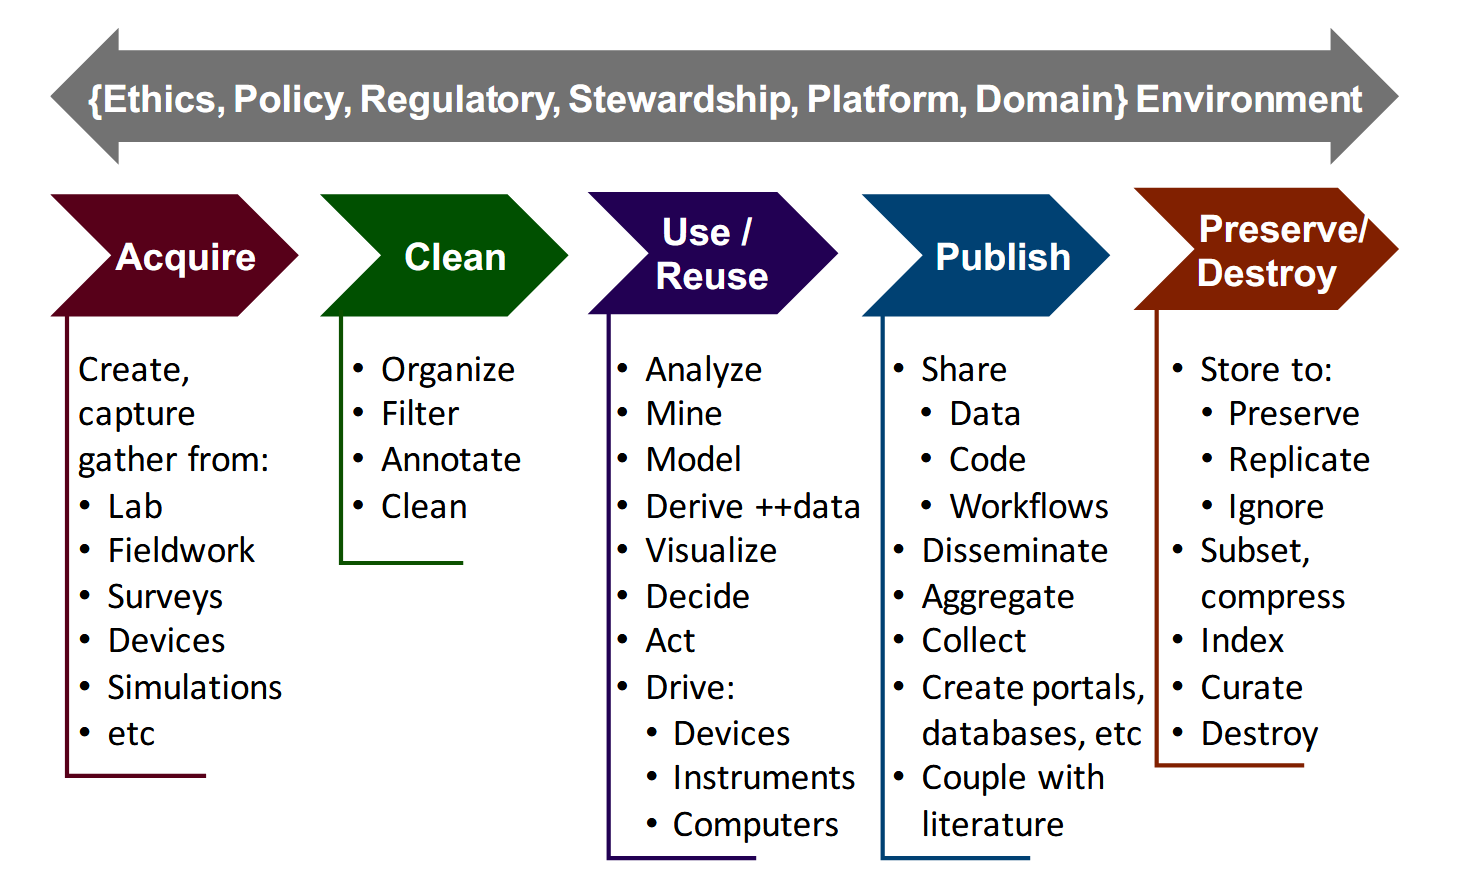
\includegraphics[width=0.8\linewidth]{figs/chapter2/datalifecycle}
	\caption{Ciclo de vida de los datos \cite{potential}}
	\label{fig:datalifecycle}
\end{figure}

Por definición, la ciencia de datos depende de los datos sobre los que se está trabajando. Por esto, el proceso de trabajo de la ciencia de datos depende generalmente del \textbf{ciclo de vida de los datos}: las distintas etapas por las que pasa un conjunto de datos desde su recolección e investigación hasta su uso final \cite{datasciencelifecycle}. Como se observa en la \textbf{Figura \ref{fig:datalifecycle}}, este ciclo está tradicionalmente dividido en \textbf{cinco} apartados \cite{potential}:



\begin{enumerate}
	\item \textbf{Adquisición:} En la actualidad, los datos se generan en cantidades masivas - del orden de \textbf{exabytes por hora} \cite{Wing2019Data}. Por tanto, el primer paso del ciclo consiste en la adquisición y almacenamiento eficiente de los datos necesarios para el proceso.
	\item \textbf{Limpieza:} Tras la adquisición, el segundo paso del ciclo consiste en la transformación de los datos originales en datos utilizables posteriormente - a través de procesos de limpieza, imputación, formateo...
	\item \textbf{Uso y re-uso:}  El tercer paso del ciclo consiste en el uso de los datos procesados con el fin de adquirir conocimiento y tomar decisiones a partir de éstos. Éste apartado se puede dividir, a su vez, en tres subapartados \cite{Wing2019Data}:
		\begin{enumerate}
			\item \textbf{Análisis exploratorio:} El estudio del comportamiento de los datos con el fin de plantear hipótesis para guiar el resto del ciclo de datos \cite{eda}.
			\item \textbf{Modelado:} El uso de técnicas computacionales y estadísticas para extraer conocimiento y predicciones a partir del conjunto de datos.
			\item \textbf{Visualización, interpretación y actuación:}  La representación gráfica de los resultados del uso de los datos, con el fin de facilitar la toma de decisiones posterior a las personas.
		\end{enumerate}
	\item \textbf{Publicación:} El cuarto paso del ciclo consiste en la diseminación de los resultados del proceso - con el fin de que el conocimiento creado pueda ser conocido y reutilizado por el mayor número de personas posible.
	\item \textbf{Preservación o destrucción:} El quinto y último paso del ciclo consiste en la preservación o destrucción de los datos utilizados - cumpliendo con otros factores como pueden ser las consideraciones éticas o regulatorias.
\end{enumerate}

Con el fin de regularizar, estandarizar y hacer reproducible el proceso completo de la ciencia de datos - desde la adquisición de los conjuntos de datos hasta la distribución de los resultados -, se han propuesto varias ampliaciones y adaptaciones del ciclo de datos estudiado, conocidas como \textbf{ciclos de vida de la ciencia de datos} \cite{datasciencelifecycle}. 

Aunque actualmente no existe un ciclo estandarizado, uno de los procesos más utilizados para ciencia de datos es el \textbf{Cross-Industry Standard Process for Data Mining (\textit{CRISP-DM})}, propuesto originalmente para el campo de la minería de datos pero adaptado a las necesidades de la ciencia de datos \cite{shearer2000crisp} - siendo el proceso utilizado a lo largo del trabajo descrito en esta memoria.

\subsection{Cross-Industry Standard Process for Data Mining - CRISP-DM}

\textbf{Cross-Industry Standard Process for Data Mining} (abreviado como \textit{CRISP-DM}) es una metodología desarrollada con el fin de ofrecer un proceso de trabajo completo de principio a fin para la minería de datos; independientemente del campo, las herramientas o la aplicación final de los datos \cite{shearer2000crisp}. Si bien fue propuesto originalmente en el año 2000, en la actualidad sigue siendo uno de los procesos más utilizados tanto en minería de datos como en ciencia de datos \cite{datasciencepmCRISPDMStill}.

\begin{figure}[h]
	\centering
	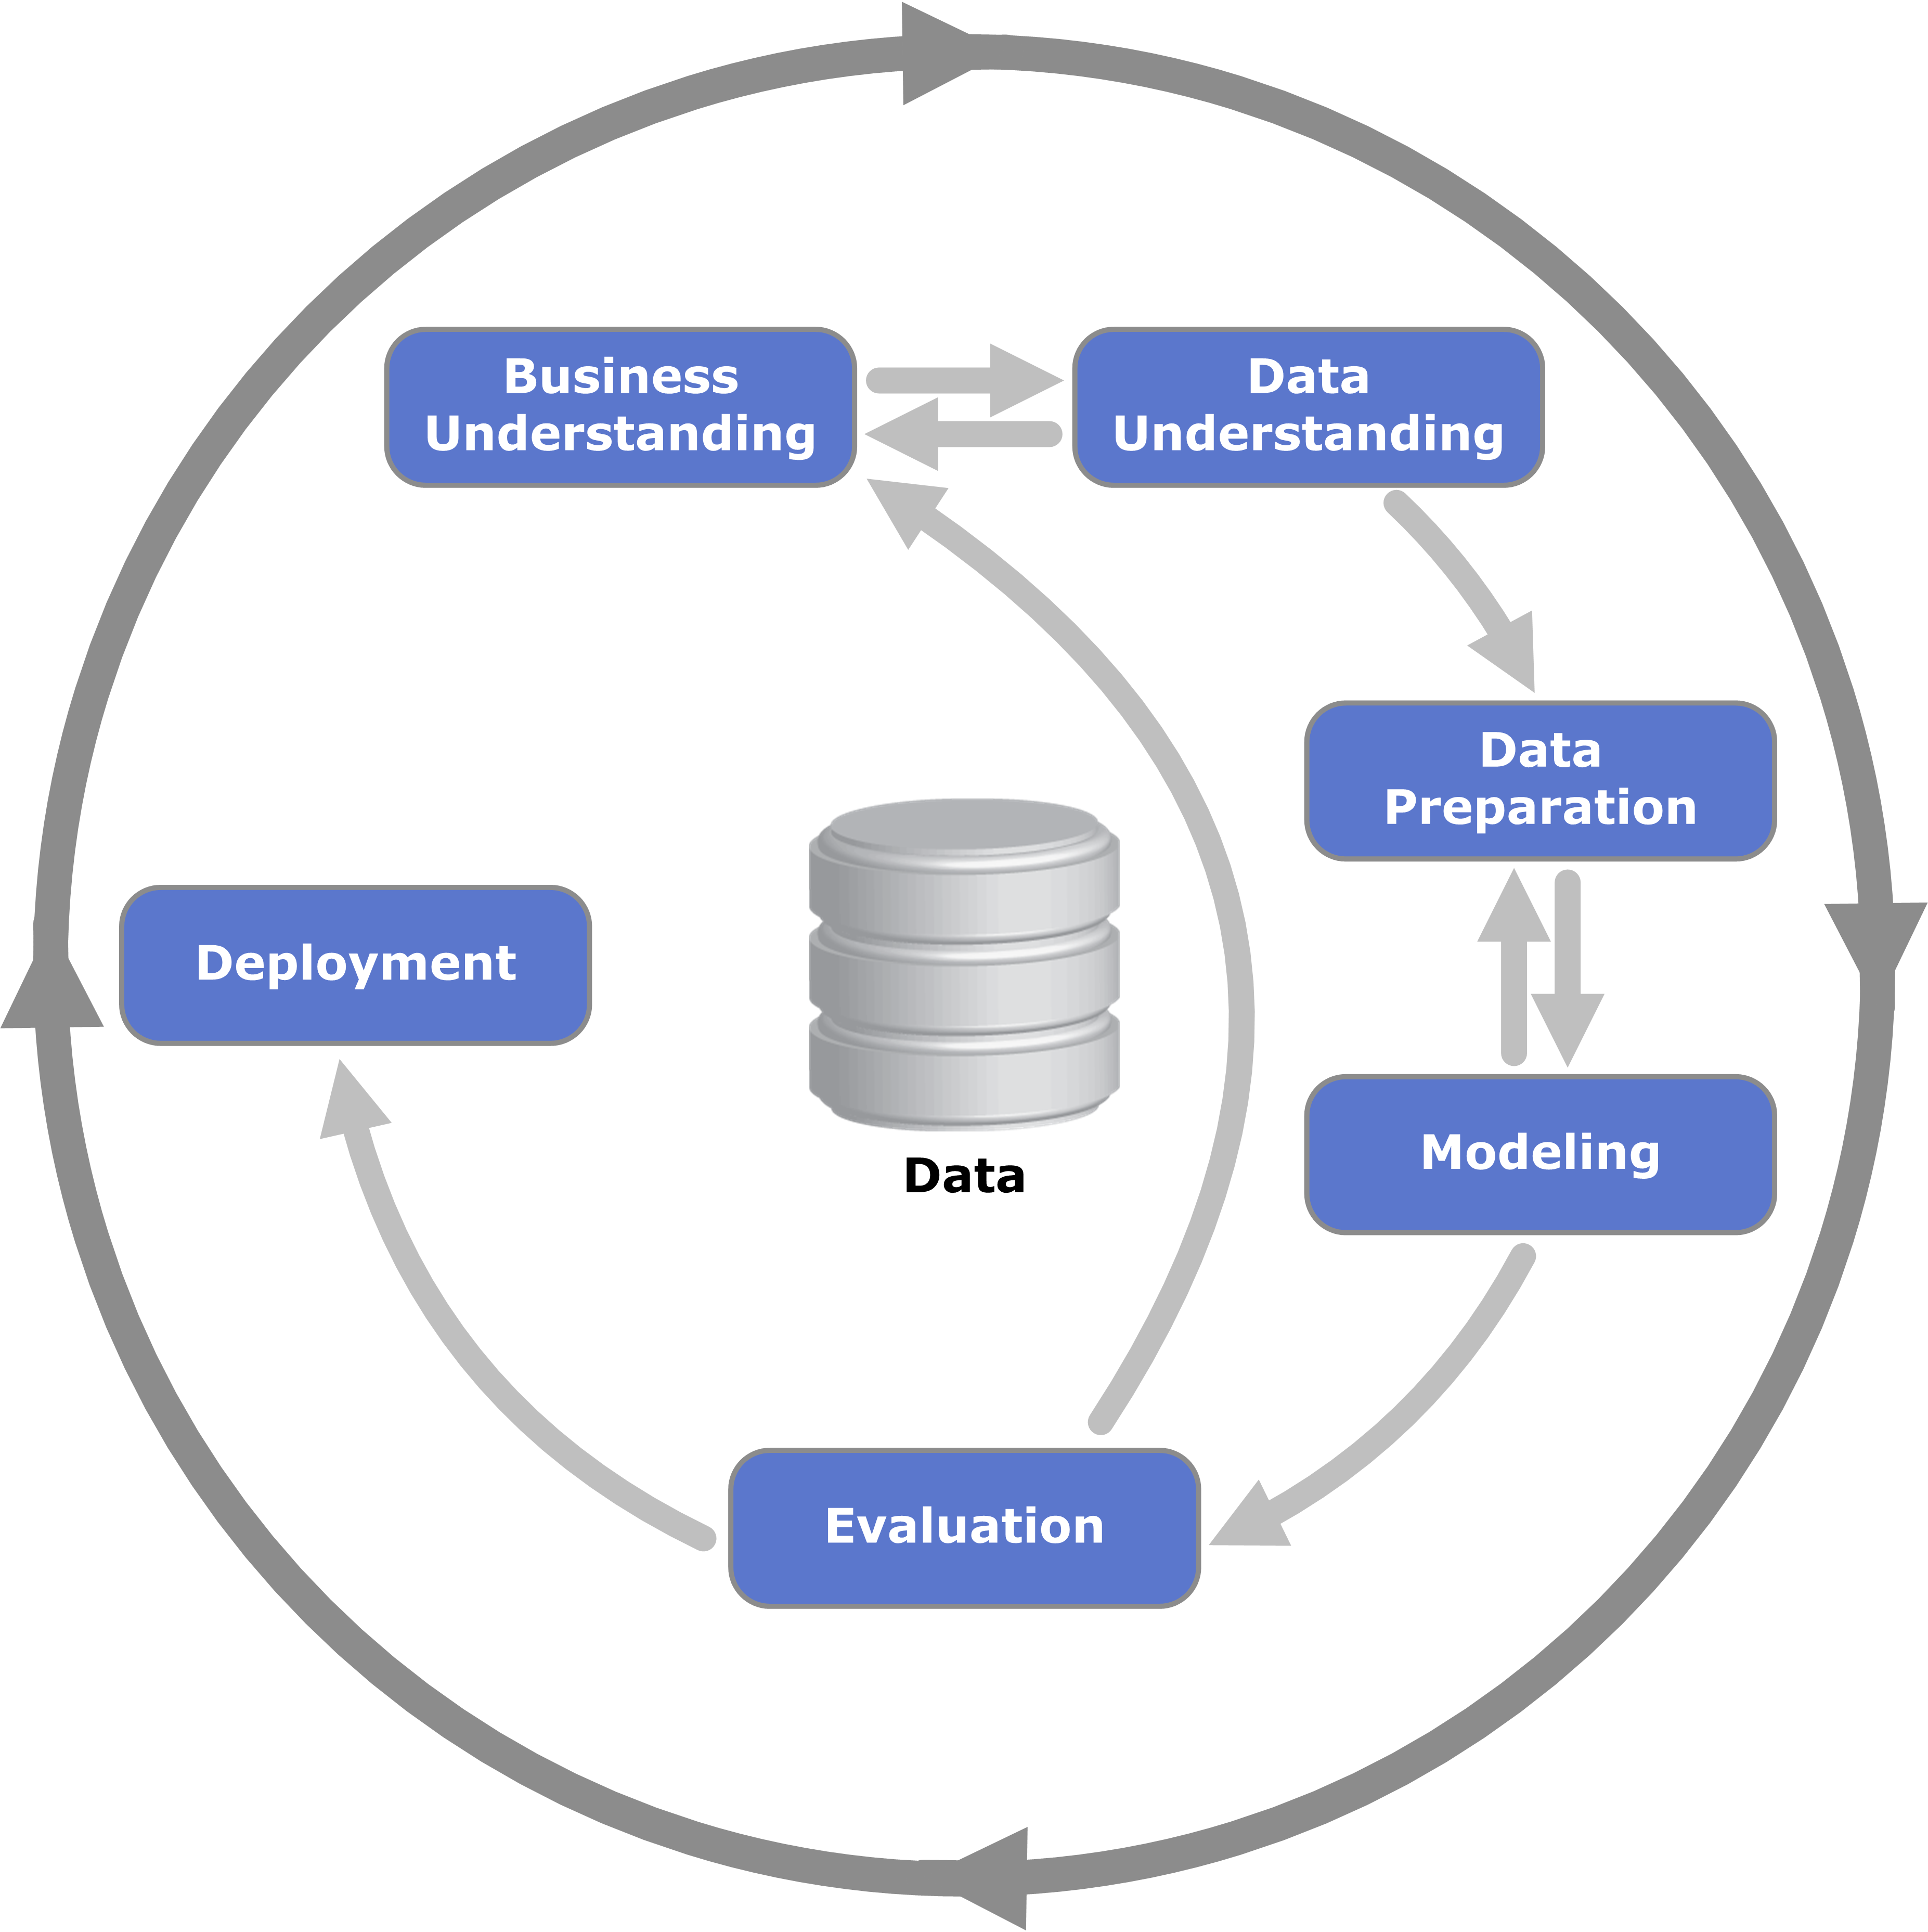
\includegraphics[width=0.6\linewidth]{figs/chapter2/crispdm}
	\caption{Ciclo de vida de CRISP-DM \cite{shearer2000crisp}}
	\label{fig:crispdm}
\end{figure}

Como se observa en la \textbf{Figura \ref{fig:crispdm}}, el ciclo de CRISP-DM está dividido en \textbf{seis fases} \cite{shearer2000crisp}, similares al ciclo de datos estudiado:

\begin{enumerate}
	\item \textbf{Conocimiento del campo (\textit{Business Understanding}):} El primer paso del ciclo consiste en entender el problema y los objetivos a resolver - estudiando la situación actual y estableciendo los pasos para alcanzar las metas propuestas.
	\item \textbf{Conocimiento de los datos (\textit{Data Understanding}):} El segundo paso del ciclo consiste en adquirir y estudiar los datos - tanto de forma superficial como en un análisis exploratorio más profundo -, además de verificar que los datos disponibles son útiles para los objetivos propuestos.
	\item \textbf{Preparación de los datos (\textit{Data Preparation}):} Tras la adquisición de conocimiento, el tercer paso consiste en preparar los datos obtenidos para su uso posterior - seleccionando las instancias relevantes, limpiando los datos para eliminar valores perdidos, enriqueciendo los datos con información externa...
	\item \textbf{Modelado (\textit{Modeling}):} Con los datos preparados, la cuarta fase del ciclo consiste en el uso y calibración de modelos de aprendizaje automático a aplicar sobre los datos - definiendo los estudios y experimentos a realizar sobre los modelos, y evaluando el rendimiento final de éstos.
	\item \textbf{Evaluación (\textit{Evaluation}):} Antes de desplegar el modelo final, la quinta fase del ciclo consiste en evaluar si los resultados obtenidos satisfacen los objetivos propuestos y si el proceso de ciencia de datos se ha aplicado de forma adecuada.
	\item \textbf{Despliegue (\textit{Deployment}):} La última fase del ciclo es el despliegue y diseminación de los resultados obtenidos - haciendo disponible el modelo y los resultados a los usuarios finales.
	
\end{enumerate}

Es importante destacar que, como indican las flechas de la \textbf{Figura \ref{fig:crispdm}}, la metodología propuesta no es linear, sino que el flujo entre los distintos pasos se puede ver alterado:
\begin{itemize}
	\item Las fases tienen dependencias entre sí - los descubrimientos en algunas fases pueden producir que sea necesario volver a fases anteriores para perfeccionar el proceso.
	\item El proceso es \textbf{cíclico} - los conocimientos adquiridos durante las distintas fases se aplican para refinar futuros procesos, ya sean sobre el mismo conjunto de datos o datos nuevos.
\end{itemize}

\section{Aprendizaje automático y ajuste de modelos}

\subsection{Aprendizaje automático}

El \textbf{aprendizaje automático} (también conocido en inglés como \textit{Machine Learning}) es una rama de la inteligencia artificial que consiste en la creación de programas capaces de \textbf{aprender} - es decir, de mejorar su rendimiento en una tarea - a través de la experiencia y de la información que se les aporta \cite{mitchell1997machine}. 

También se puede definir el término como el conjunto de métodos capaces de detectar patrones en los datos de forma autónoma, y de utilizar dichos patrones para predecir datos futuros \cite{mlprobabilistic} - siendo este último de mayor interés a los principios de la ciencia de datos.

Generalmente, los algoritmos de aprendizaje automático se dividen en dos grandes familias, en función del tipo de datos e información que se aporta a los algoritmos \cite{aima} \cite{mlprobabilistic}:

\begin{itemize}
	\item \textbf{Aprendizaje supervisado:} El objetivo del algoritmo es aprender una función capaz de, dados unos datos de entrada $X$, predecir una salida $Y$. Esta función se aprende a partir de un conjunto de datos $D={(x_i, y_i)}^{N}_{i=1}$ donde a cada instancia $x_i$ del conjunto de datos $D$ se le asocia un valor esperado $y_i$.
	
	Este tipo de aprendizaje se puede dividir a su vez en dos categorías dependiendo del tipo de salida $Y$ que se espera \cite{aima}:
	\begin{itemize}
		\item \textbf{Clasificación}: El algoritmo busca obtener para cada entrada $x_i$ un valor concreto \textbf{dentro de un conjunto finito de posibles valores}.
		\item \textbf{Regresión}: El algoritmo busca obtener, para cada entrada $x_i$, un \textbf{valor numérico continuo}.
	\end{itemize}
	\item \textbf{Aprendizaje no supervisado:} El objetivo del algoritmo es aprender patrones subyacentes de los datos de entrada $X$ ofrecidos, sin buscar predecir una salida. Esta función se aprende a partir de un conjunto de datos $D={x_i}^{N}_{i=1}$ donde no se ofrece ningún tipo de etiqueta a cada instancia $x_i$.
\end{itemize}

Un \textbf{modelo} es el resultado del proceso de aprendizaje automático: una función capaz de predecir una salida para una entrada dada, y cuyos parámetros e hiperparámetros han sido ajustados a través de un entrenamiento sobre un conjunto de datos para \textbf{minimizar un error} \cite{Burkov2019TheHM}. 

De cara a cumplir el objetivo propuesto por el trabajo descrito en esta memoria - la creación de un modelo capaz de \textbf{predecir el tiempo de diagnóstico} -, se van a trabajar con modelos supervisados de \textbf{regresión}. Por esto, resulta de interés describir los principales modelos a utilizar y el ajuste que se va a realizar sobre ellos.

\subsection{Selección de modelos}

Durante el entrenamiento de los modelos, se pueden encontrar algunos problemas:
\begin{itemize}
	\item Se han entrenado varios modelos, y es necesario elegir de forma objetiva uno de ellos en base a su rendimiento.
	\item Se necesitan elegir los hiperparámetros de un modelo que mejor rendimiento ofrecen sobre el conjunto de datos, de forma objetiva.
	\item Los modelos entrenados han aprendido variaciones insignificantes y patrones falsos - ruido interpretado como información real - a partir de los datos de entrada, llevando a un problema de \textbf{sobreajuste} \cite{mlprobabilistic} que puede afectar de forma negativa al rendimiento del modelo.
\end{itemize}

En estos casos, nos interesa seleccionar de entre todos los modelos a evaluar el modelo más \textbf{generalizable} - es decir, el modelo que tendría el \textbf{menor error esperado} si se evaluase con un conjunto de datos distinto al utilizado durante el entrenamiento \cite{mlprobabilistic}. 

Ahora bien, a la hora de la verdad no es común tener acceso a dicho hipotético conjunto de test - o si se tiene, solo debería ser utilizado para evaluar el rendimiento del modelo seleccionado finalmente para evitar que se sesgue la selección de modelos \cite{aima}. 

Para solucionar este problema y realizar una selección de modelos \textbf{honesta}, se pueden utilizar las siguientes opciones \cite{mlprobabilistic}:

\begin{itemize}
	\item \textbf{Conjunto de validación:} Se particiona el conjunto de datos inicial en entrenamiento y validación - utilizando el primero para entrenar los modelos, y el segundo para evaluar su rendimiento honesto y seleccionar el modelo.
	\item \textbf{K-Validación cruzada:} En caso de que el conjunto de datos no sea suficientemente grande para particionarse, se puede optar por particionar el conjunto de datos en \textbf{K trozos} de igual tamaño. Para cada uno de estas particiones, se entrenan los modelos con el resto de particiones y se evalúan los rendimientos sobre la partición seleccionada. Tras realizar este proceso $K$ veces, se puede utilizar el error promedio de los $K$ entrenamientos como una aproximación al rendimiento honesto del modelo para realizar la selección.
\end{itemize}

\subsection{Modelos de regresión}

En el caso de la \textbf{regresión}, el objetivo del modelo es aprender una función capaz de predecir un valor numérico continuo para cada instancia de datos de entrada \cite{mlprobabilistic}. Dicha función se ajusta buscando encontrar el conjunto de parámetros que \textbf{minimiza} la diferencia entre los valores predichos por la función y los valores reales asociados a los datos de entrada \cite{Burkov2019TheHM}.

Se han propuesto y estudiado un gran número de modelos de regresión, con parametrizaciones y funcionamientos diversos, en la bibliografía \cite{tai2021surveyregressionalgorithmsconnections}. Pese a esta variedad, es posible dividir todas estas familias de modelos en dos grandes grupos: modelos \textbf{tradicionales} y modelos de \textbf{conjuntos o \textit{ensembles}} \cite{aima}

\subsubsection{Modelos tradicionales - regresión lineal, árboles de decisiones y máquinas de vectores de soporte}

Si bien no hay una definición consensuada sobre su definición, se puede entender como \textbf{modelo tradicional} a un modelo que entrena una única función con el fin de realizar predicciones sobre la salida esperada para cada entrada de datos \cite{aima}.

Existe una gran cantidad de familias de modelos con una larga trayectoria en la bibliografía existente \cite{Burkov2019TheHM}. Ahora bien, el estudio realizado en la memoria se centra en las siguientes tres familias de modelos utilizadas en el trabajo:

\begin{itemize}[leftmargin=*]
	\item \textbf{Regresión lineal:} 
	
	Los modelos más simples, trabajando con la suposición de que \textbf{existe una correlación lineal} entre los atributos de entrada y la salida del modelo \cite{mlprobabilistic}. Por lo general, la salida $y$ para una entrada $x$ se predice utilizando la siguiente fórmula: 

	$$y(x) = \sum_{j=1}^{D}w_j x_j$$
	
	Donde $x_j$ representa cada atributo de la entrada y $w_j$ el peso asignado a cada atributo, siendo el objetivo de estos modelos ajustar los pesos asignados a cada atributo para minimizar el error cuadrado \cite{aima}. Ahora bien, cuando se trabaja con conjuntos de datos de gran dimensionalidad, el gran número de atributos puede afectar de forma negativa al rendimiento del modelo, causando un sobreajuste al conjunto de entrenamiento \cite{l1l2}.
	
	Para evitar este problema, se proponen técnicas de \textbf{regularización} - penalizaciones aplicadas a la fórmula del error con el objetivo de conseguir modelos menos complejos y más generalizables \cite{elasticnet}. Los tres modelos de regularización más utilizados son los siguientes:
	
	\begin{itemize}
		\item \textbf{Ridge (L2) \cite{ridge}:} Como factor de penalización, se utiliza $\sum_{j=1}^D(w_j)^2$ - la suma de los pesos cuadrados del modelo, buscando reducir de forma generalizada la influencia de los atributos para evitar sobreajustes y correlaciones.
		\item \textbf{Lasso (L1) \cite{lasso}:} Como factor de penalización, se utiliza $\sum_{j=1}^D|w_j|$ - la suma del valor absoluto de los pesos del modelo, buscando eliminar los atributos irrelevantes reduciendo su peso a $0$.
		\item \textbf{Elastic-Net \cite{elasticnet}:} Como factor de penalización, se utiliza $\lambda\left(\sum_{j=1}^D(w_j)^2\right) + (1-\lambda)\left(\sum_{j=1}^D|w_j|\right)$ - utilizando a la vez las regularizaciones L1 y L2 de forma ponderada, buscando aunar los beneficios de ambas aproximaciones.
	\end{itemize}

	\item \textbf{Máquinas de vectores de soporte (SVM):} 
	
	Las máquinas de vectores de soporte se pueden entender como una evolución de los modelos de regresión lineal donde, en vez de buscar la linea que mejor se ajusta al conjunto de datos, se busca el \textbf{hiperplano} capaz de ajustarse al conjunto de datos con el \textbf{mayor margen} \cite{aima}. 
	
	En regresión, esto se traduce en la búsqueda de la función representando al mejor hiperplano capaz de ajustarse a todas las instancias del conjunto de datos a la vez que es capaz de mantener una distancia inferior a un margen $\epsilon$ con todos los puntos \cite{svr}.
	
	La principal utilidad de estos modelos radica en las dos siguientes características \cite{aima}:
	\begin{itemize}
		\item \textbf{Funciones kernel:} Un problema de los modelos lineales es que los conjuntos de datos no siempre son linealmente separables. Para solventar este problema, las máquinas de vectores de soporte son capaces de utilizar \textbf{funciones \textit{kernel}} para transformar los datos a una mayor dimensionalidad - donde si es posible ajustar un hiperplano con mayor margen.
		\item \textbf{Vectores de soporte:} Para definir el modelo no es necesario almacenar información sobre el conjunto de datos completo, sino que es suficiente con almacenar información sobre los \textbf{puntos que definen la frontera entre el hiperplano y el margen} - conocidos como los vectores de soporte.
	\end{itemize}
	
	\item \textbf{Árboles de decisión:} 
	
	Los árboles de decisión son modelos de reglas representando su función a través de grafos dirigidos \cite{Burkov2019TheHM} donde la predicción se obtiene realizando una serie de comprobaciones secuenciales empezando desde la raíz, ramificando hasta llegar a una hoja final \cite{aima}. Estos árboles se dividen en los siguientes componentes:
	
	\begin{itemize}
		\item \textbf{Nodos:} Nodos internos del árbol donde se realiza una comprobación sobre el valor de un atributo. Dependiendo del resultado de la comprobación, el nodo se \textbf{ramifica} a otros nodos u hojas.
		\item \textbf{Hojas:} El valor final predicho para una entrada, alcanzado tras una serie de comprobaciones en nodos.
	\end{itemize}
	
	El objetivo del modelo es, por tanto, aprender el conjunto de reglas que minimiza el error del modelo para el conjunto de datos dado. Ahora bien, estos modelos tienden a \textbf{sobreajustar} creando árboles de gran profundidad \cite{aima}.

\end{itemize}

\subsubsection{Modelos de ensemble - bagging y boosting}

Como contraste a los modelos tradicionales, un \textbf{modelo de conjunto, meta-modelo o \textit{ensemble}} es un modelo que, durante su entrenamiento, ha aprendido un \textbf{conjunto de funciones o modelos sencillos} - por lo general, una agrupación de modelos tradicionales -, agrupando las predicciones de todos éstos para obtener una predicción general de la salida esperada para cada entrada de datos \cite{aima}.

Los algoritmos de \textit{ensemble} buscan aprender un gran número de modelos simples con rendimiento ligeramente mejor que un modelo aleatorio - conocidos como \textbf{modelos de aprendizaje débil}, generalmente \textbf{árboles de decisión} \cite{Burkov2019TheHM}. Suponiendo que cada uno de estos modelos es completamente independiente al resto, la unión de sus resultados lleva a una predicción final \textbf{más precisa y generalizable} que un único modelo entrenado \cite{Burkov2019TheHM}.

Dependiendo de la metodología utilizada para entrenar los modelos simples - ya sea de forma secuencial o paralela -, se pueden dividir los algoritmos en dos familias \cite{aima}:


\begin{itemize}

	\item \textbf{Bootstrap Aggregating (Bagging):} 
	
	Los modelos de \textit{ensemble} trabajan con la suposición de que cada uno de los modelos individuales que lo componen es totalmente independiente al resto de modelos. Ahora bien, en la práctica no suele ser factible entrenar a cada modelo individual sobre un conjunto de datos independiente \cite{baggingart}. 
	
	Para solventar este problema, los modelos de \textbf{\textit{bagging}} entrenan cada modelo sobre una \textbf{muestra uniformemente aleatoria con reemplazo} (\textit{bootstrap} en inglés) del conjunto de datos original \cite{baggingart} - obteniendo como resultados modelos sencillos e independientes, y siendo la predicción final el \textbf{promedio} de las predicciones de cada modelo.

	Algunos de los modelos de \textit{bagging} más importantes son los siguientes:
	
	\begin{itemize}
		\item \textbf{\textit{Random Forest} \cite{randomforests}:} Un modelo de \textit{ensemble bagging} de \textbf{árboles de decisión profundos} en el que se añade un segundo proceso de muestreo aleatorio para aumentar la independencia entre los predictores simples entrenados:
		\begin{itemize}
			\item \textbf{Muestreo de instancias:} Cada árbol se entrena con un subconjunto aleatorio de instancias del conjunto de datos.
			\item \textbf{Muestreo de atributos:} Cada árbol se entrena con un subconjunto aleatorio de atributos del conjunto de datos.
		\end{itemize}
		\item \textbf{\textit{Extremely Randomized Trees \cite{Geurts2006}:}} Una evolución del modelo de \textit{Random Forest} en el que se añade un proceso de muestreo adicional, con los siguientes cambios:
		\begin{itemize}
			\item Cada árbol pasa a entrenarse sobre el \textbf{conjunto de datos completo}, sin muestreo - aunque se sigue realizando un muestreo de los atributos a considerar por cada árbol.
			\item Durante la construcción del árbol, se generan de forma aleatoria varias \textbf{particiones del conjunto de datos} para cada atributo - en vez de calcular la partición óptima. A la hora de construir cada nodo, se elige la partición que mejor puntuación obtiene de todas las generadas.
		\end{itemize}
	\end{itemize}
	
	\item \textbf{Boosting:}
	
	Para garantizar la independencia entre los modelos entrenados, los modelos de \textit{ensemble} de tipo \textbf{boosting} optan por entrenar sus modelos de forma \textbf{secuencial} sobre un \textbf{conjunto de datos con pesos} - donde, para cada modelo, se da más peso a las instancias del conjunto de datos que se han predicho erróneamente en los modelos anteriores \cite{aima}.
	
	Durante el trabajo, se ha considerado el siguiente modelo de \textit{boosting}:
	
	\begin{itemize}
		\item \textbf{\textit{Adaptive Boosting \cite{adaboost}:}} Un modelo básico de \textit{boosting} que sigue estrictamente el proceso descrito. Concretamente, se comienza con un conjunto de datos de pesos uniformes sobre el que se entrena el primer modelo, ajustando los pesos de las instancias - aumentando el peso de las instancias con mayor error, y reduciendo el peso de las instancias con menor error. Tras esto, se repite el proceso de entrenamiento de modelos y ajuste de pesos hasta entrenar todos los predictores \cite{aima}.
		
		La predicción final es una \textbf{media ponderada por el error} de la predicción de todos los modelos - donde los modelos con menor error tienen un mayor peso en la ponderación.
	\end{itemize}
	
	Una subfamilia dentro de estos algoritmos son los modelos de \textbf{Gradient Boosting}. Estos modelos también utilizan la metodología de \textit{boosting} - entrenar modelos secuencialmente ajustándose a los errores del modelo anterior -, con la diferencia de que el entrenamiento no se hace sobre el conjunto de datos directamente, sino sobre los \textbf{errores residuales} (la diferencia entre la predicción y el valor real) de cada instancia \cite{gradientboosting}. 
	
	Este comportamiento es similar al \textbf{gradiente descendiente} utilizado para entrenar otros modelos como la regresión lineal o las redes neuronales \cite{Burkov2019TheHM}. En concreto, se llevan a cabo los siguientes pasos:
	\begin{enumerate}
		\item Se comienza realizando una predicción inicial, generalmente el valor promedio de todas las instancias.
		\item Utilizando el valor estimado, se calculan los \textbf{errores pseudo-residuales} de cada instancia - el \textbf{error} entre la predicción y el valor real. Estas pseudo-residuales dependen de la función de error que se elija.
		\item Repitiéndose para cada modelo que se tiene que entrenar:
		\begin{enumerate}
			\item A partir de los valores pseudo-residuales, se entrena un modelo simple que \textbf{predice el valor residual de cada instancia}.
			\item Utilizando los nuevos residuales estimados, se recalculan los valores pseudo-residuales para que el siguiente modelo ajuste mejor a las instancias clasificadas erroneamente.
		\end{enumerate}
	\end{enumerate}
	
	Para obtener una predicción final, se suma al valor promedio inicial los residuales calculados por cada uno de los modelos - ponderados por un \textbf{factor de aprendizaje} para evitar el sobreajuste \cite{gradientboosting}.
	
	Actualmente, los modelos de \textit{Gradient Boosting} son considerados el estado del arte para la mayoría de problemas de predicción estructurada \cite{Burkov2019TheHM}, siendo algunos de los modelos más populares los siguientes:
	
	\begin{itemize}
		\item \textbf{\textit{Extreme Gradient Boosting \cite{Chen_2016}:}} Un algoritmo de \textit{Gradient Boosting} utilizando el método de Newton-Raphson - en vez de calcular los errores pseudo-residuales, se calcula una función de la segunda y la primera derivada de la función de error. Además, el modelo está diseñado para permitir el entrenamiento en paralelo de los árboles.
		\item \textbf{\textit{Categorical Boosting \cite{dorogush2018catboostgradientboostingcategorical}:}} Un algoritmo de \textit{Gradient Boosting} diseñado para trabajar de forma nativa con atributos categóricos sin necesidad de convertirlos previamente a valores numéricos. 
		
		El modelo se entrena utilizando \textbf{\textit{Ordered Boosting}} - utilizando una permutación aleatoria del conjunto de entrenamiento para cada modelo, donde para calcular las pseudo-residuales de cada instancia se consideran solo las instancias anteriores en la permutación \cite{catboost2} - para evitar introducir sesgos.
		\item \textbf{\textit{Light Gradient-Boosting Model \cite{NIPS2017_6449f44a}:}} Un algoritmo de \textit{Gradient Boosting} con las siguientes características:
		\begin{itemize}
			\item \textbf{Histogramas:} Para optimizar el rendimiento, los valores de los atributos continuos se agrupan en histogramas.
			\item \textbf{Crecimiento del arbol por hojas:} Frente a otros algoritmos que entrenan los árboles nivel a nivel, el modelo ramifica siempre por la hoja que minimizaría el error - llevando a árboles más ajustados.
		\end{itemize}
		
		Existe otra implementación de este algoritmo, conocida como \textbf{Histogram-Based Gradient Boosting}, ofrecida por la librería de ciencia de datos \textit{Scikit-Learn} \cite{scikit-learn} - aunque ambas se basan en el mismo modelo y no presentan diferencias significativas.
	\end{itemize}
\end{itemize}



% 3 - EDA del conjunto de datos
\chapter{Estudio exploratorio del problema}

En este capítulo se estudia en detalle el problema a resolver a través del proceso de ciencia de datos. Se comienza realizando una definición del problema y sus objetivos, seguido por un \textbf{análisis exploratorio de los datos} que lo definen. En este análisis se estudian los atributos que describen los datos junto a sus distribuciones y comportamientos - haciendo hincapié en los atributos de carácter geográfico, social y económico.

\section{Definición y objetivos del problema}

El \textbf{cáncer de mama triple negativo} es uno de los cánceres de mama más agresivos y difíciles de tratar. En el caso de que además se agravase con una \textbf{metástasis}, se necesita un tratamiento rápido y urgente, sin retrasos innecesarios, para aumentar al máximo las posibilidades de éxito. Ahora bien, el tiempo de espera para acceder a dicho tratamiento no es igual para todos los pacientes, y existe la posibilidad de que hayan sesgos influyendo en el tiempo de diagnóstico - como pueden ser algunos factores geográficos, socioeconómicos o incluso climáticos \cite{widsdatathon2024-challenge2}.

El principal objetivo del problema - y, por tanto, el objetivo que guía el proceso de ciencia de datos - es \textbf{crear un modelo de regresión} capaz de predecir el tiempo de diagnóstico de metástasis en base a la información dada de un paciente. Además, se busca estudiar la \textbf{influencia de factores geográficos, socioeconómicos y climáticos} en dicho tiempo de diagnóstico, para comprobar si existe un sesgo real en el trato a los pacientes.
El problema a resolver se planteó originalmente como el segundo de los desafíos ofrecidos por la institución \textbf{Women in Data Science} como parte de su \textit{Datathon} de 2024 \cite{widsdatathon2024-challenge2}.

\section{Análisis exploratorio de datos}

El primer paso en el proceso de ciencia de datos es realizar un estudio exhaustivo del conjunto de datos con el fin de comprender mejor su comportamiento y la distribución de sus datos.

\subsection{Distribución del conjunto de datos}

El conjunto de datos contiene un total de \textbf{13173 instancias}, cada una de ellas descrita por \textbf{150 atributos} - divididos en \textbf{11 atributos categóricos} y \textbf{139 atributos numéricos} - y una \textbf{variable objetivo numérica}. Describir individualmente todos los atributos en la memoria no sería factible, por lo que se describen los principales grupos de atributos:

\begin{itemize}
	\item \textbf{Atributos médicos (13 atributos - 11 categóricos y 2 numéricos)}: Datos identificativos e información sobre el diagnóstico, tratamiento y seguro del paciente.
	\item \textbf{Atributos socioeconómicos (65 atributos - 2 categóricos y 63 numéricos)}: Por lo general, datos \textbf{estadísticos} reflejando información socioeconómica relacionada con la población del paciente. Estos estadísticos se pueden dividir, a su vez, en:
	\begin{itemize}
		\item \textbf{Porcentajes (49 atributos numéricos):} Porcentajes en el rango $[0, 100]$ representando valores estadísticos - matrimonios, educación, demografía... - de la ubicación del paciente.
		\item \textbf{Medianas (10 atributos numéricos):} Valores representando la mediana de algunos estadísticos - edad, ingresos, alquileres... - de la ubicación del paciente.
		\item \textbf{Información geográfica (6 atributos - 2 categóricos y 4 numéricos):} Valores concretos - población, densidad... - de la ubicación del paciente, sin ser representados a través de un porcentaje o una mediana.
	\end{itemize}
	\item \textbf{Atributos climáticos (72 atributos numéricos)}: Temperatura promedio (en grados \textbf{Farenheit}) de la población del paciente - representada de forma mensual entre los años 2013 y 2018.
\end{itemize}

\subsubsection{Variable objetivo - tiempo de diagnóstico}

La variable objetivo - el \textbf{tiempo de diagnóstico de una metástasis} - es una variable \textbf{numérica entera} con valores en el conjunto de entrenamiento en el rango $[0-365]$, cuya distribución se puede observar en la \textbf{Figura \ref{fig:ch3varobjetivo}}.

\begin{figure}[h]
	\begin{center}
		\begin{subfigure}{0.45\linewidth}
			\begin{center}
				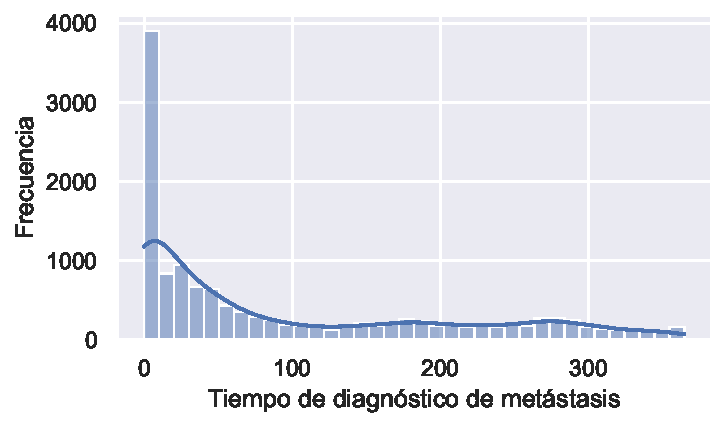
\includegraphics[width=\linewidth]{figs/chapter3/objectivevariable/diagnosisperioddistribution.pdf}
				\caption{Distribución general}\label{fig:ch3general}
			\end{center}
		\end{subfigure} 
		\begin{subfigure}{0.45\linewidth}
			\begin{center}
				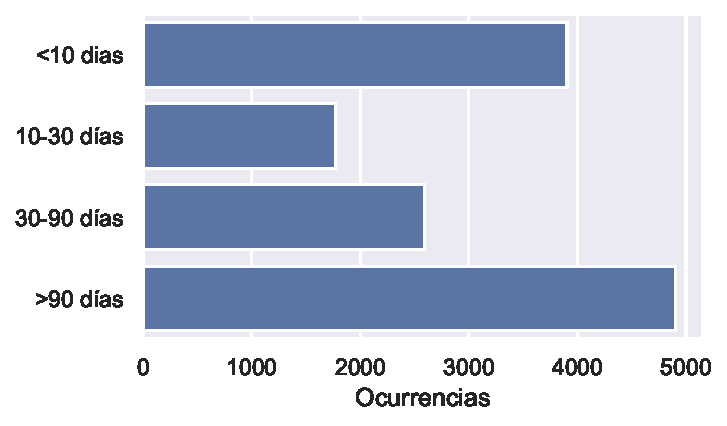
\includegraphics[width=\linewidth]{figs/chapter3/objectivevariable/diagnosisperiodgrouped.pdf}
				\caption{Distribución agrupada}\label{fig:ch3group}
			\end{center}
		\end{subfigure} 
	\end{center}
	\captionsetup{aboveskip=-5pt, belowskip=-15pt}
	\caption{Distribución del tiempo de diagnóstico}
	\label{fig:ch3varobjetivo}
\end{figure}

Se puede ver que los tiempos de diagnóstico siguen una \textbf{distribución de Poisson} - con la mayoría de casos diagnosticados en un rango de $[0-10]$ días. Ahora bien, como se observa en la \textbf{Figura \ref{fig:ch3group}}, si se agrupan los valores en rangos \textbf{la mayoría de casos tardan más de 90 días en ser diagnosticados}.

\subsubsection{Valores perdidos}

Antes de realizar un estudio más exhaustivo de los atributos, es de interés estudiar el comportamiento de los \textbf{valores perdidos} en el conjunto de datos - para comprobar si hay un gran número de éstos, si existen atributos irrelevantes por tener un alto grado de información perdida y si sería necesario realizar algún tipo de tratamiento sobre éstos valores.

\begin{figure}[h]
	\centering
	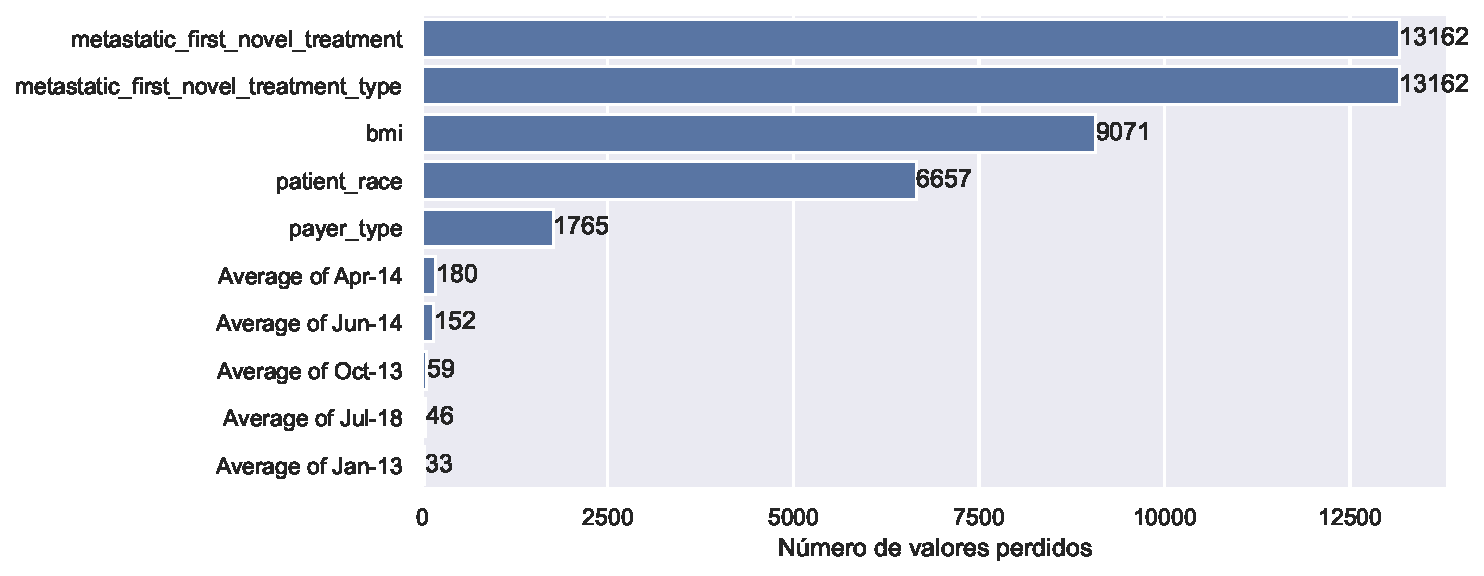
\includegraphics[width=\linewidth]{figs/chapter3/missingvalues}
	\captionsetup{belowskip=-15pt}
	\caption{Distribución de valores perdidos en el conjunto de datos}
	\label{fig:ch3missingvalues}
\end{figure}

Estudiando la distribución, \textbf{72} de los 150 atributos disponibles presentan valores perdidos - con un promedio de \textbf{624 instancias perdidas} por atributo. En primera instancia puede parecer un número muy elevado de valores perdidos, si se observa cómo se distribuyen los valores perdidos - como se representa en la \textbf{Figura \ref{fig:ch3missingvalues}} - se puede observar un \textbf{sesgo} claro, donde la amplia mayoría de valores perdidos se agrupan alrededor de cinco atributos:

\begin{itemize}
	\item \textbf{Tratamiento:} Debido al número tan elevado de valores perdidos en ambos atributos, \textbf{solo se tiene información sobre el tratamiento de 11 pacientes} - lo que significa que no sería relevante el atributo debido a la falta de información.
	\item \textbf{Índice de masa corporal del paciente:} Se conoce el índice de masa corporal de \textbf{menos de la mitad de los pacientes.}  Además, al ser información numérica \textbf{no existe un valor por defecto} por el que se puedan reemplazar los valores perdidos - por lo que sería razonable no estudiar en más detalle el atributo.
	\item \textbf{Raza y tipo de seguro médico del paciente:} En ambos casos hay un número considerable de instancias con valores desconocidos. Ahora bien y a diferencia del IMC, al ser atributos categóricos puede considerar que \textbf{es significativo para el estudio que no se conozcan estos valores} - tratándolos como una categoría adicional, \textit{"Desconocido"}.
\end{itemize}

En el resto de atributos el número de valores perdidos es más reducido - en el orden de \textbf{100 instancias} o menor -, por lo que el tratamiento es más simple, pudiendo descartar las instancias con valores perdidos o realizando una imputación simple con el valor promedio.

\subsection{Estudio de atributos categóricos}

Tras un primer análisis - en el que se ha estudiado la distribución de la variable objetivo, los atributos y sus valores perdidos -, la segunda parte del análisis exploratorio es realizar un \textbf{estudio exhaustivo individualizado} de los atributos de interés y su relación con la variable predictora. Al ser reducido el número de atributos categóricos (con un total de \textbf{11}) es posible realizar un análisis individual de cada uno de estos atributos:

\subsubsection{Datos personales - raza, género y tipo de seguro del paciente}

\begin{itemize}[leftmargin=*]
	\item \textbf{Raza del paciente:}
	
	Como se ha comentado durante el estudio de los valores perdidos, hay \textbf{un número significativo de valores perdidos} de este atributo - que serán tratados como una categoría adicional, \textit{"Unknown"}.
	
	\begin{figure}[h]
		\begin{center}
			\begin{subfigure}{0.45\linewidth}
				\begin{center}
					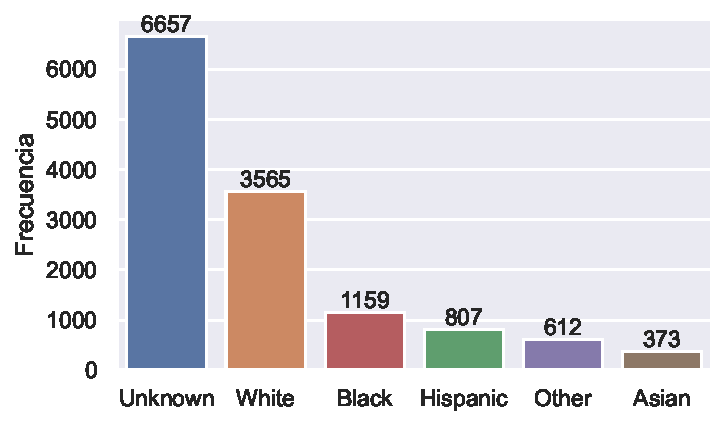
\includegraphics[width=\linewidth]{figs/chapter3/categorical/racedistribution.pdf}
					\caption{General}\label{fig:ch3racedist}
				\end{center}
			\end{subfigure} 
			\begin{subfigure}{0.45\linewidth}
				\begin{center}
					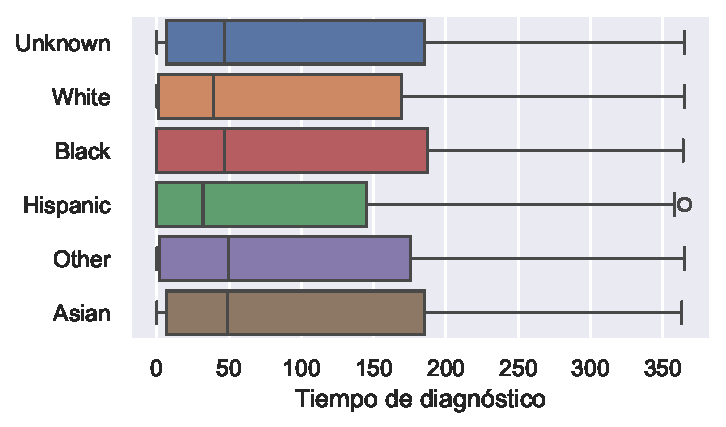
\includegraphics[width=\linewidth]{figs/chapter3/categorical/raceperiod.pdf}
					\caption{Respecto al tiempo de diagnóstico}\label{fig:ch3raceperiod}
				\end{center}
			\end{subfigure} 
		\end{center}
		\captionsetup{aboveskip=-5pt, belowskip=-15pt}
		\caption{Distribución de la raza del paciente}
		\label{fig:ch3race}
	\end{figure}
	
	
	
	En la \textbf{Figura \ref{fig:ch3race}} se puede observar que:
	\begin{itemize}
		\item \textbf{Distribución general:} Como se podía esperar, la mayoría de pacientes presentan una raza desconocida - algo que se puede interpretar como que \textbf{la mayoría de los pacientes no se sienten cómodos especificando su raza}. Tras esto, la raza \textbf{blanca} es la más frecuente - siendo tres veces más frecuente que la raza negra -, siendo la raza asiática la menos frecuente.
		\item \textbf{Relación con el tiempo de diagnóstico:} Si bien todas las razas tienen un rango de tiempos de diagnóstico amplio, \textbf{las razas blanca e hispánica tienen una mediana ligeramente inferior al resto} - sugiriendo que \textbf{la raza puede influir en el tiempo de diagnóstico}.
	\end{itemize}
	
	Dada estas observaciones, puede resultar de interés considerar la raza del paciente a la hora de hacer una selección de atributos.
	
	\item \textbf{Tipo de seguro médico del paciente:}
	
	Igual que con la raza, hay una cantidad significativa de valores perdidos de este atributo - que serán categorizados como un nuevo valor, \textit{"UNKNOWN"}.
	
	\begin{figure}[h]
		\begin{center}
			\begin{subfigure}{0.45\linewidth}
				\begin{center}
					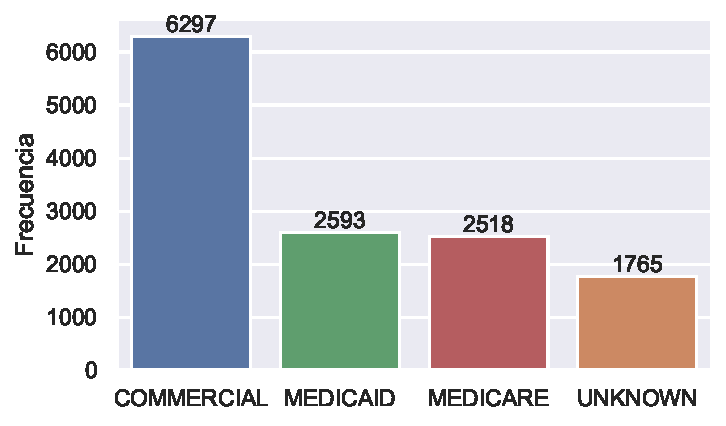
\includegraphics[width=\linewidth]{figs/chapter3/categorical/payertypedistribution.pdf}
					\caption{General}\label{fig:ch3payertypedist}
				\end{center}
			\end{subfigure} 
			\begin{subfigure}{0.45\linewidth}
				\begin{center}
					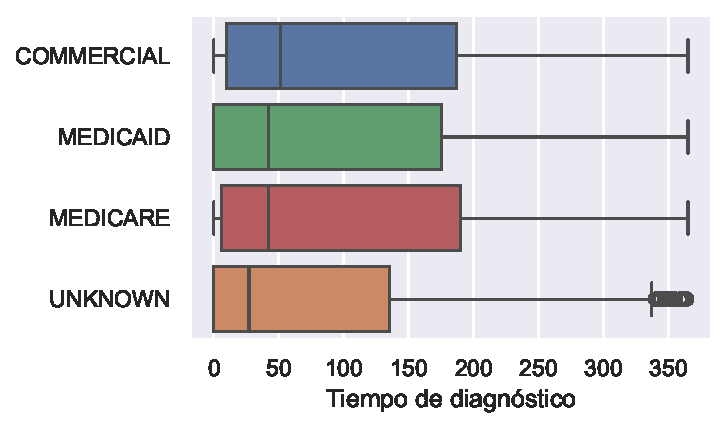
\includegraphics[width=\linewidth]{figs/chapter3/categorical/payertypeperiod.pdf}
					\caption{Respecto al tiempo de diagnóstico}\label{fig:ch3payertypeperiod}
				\end{center}
			\end{subfigure} 
		\end{center}
		\captionsetup{aboveskip=-5pt, belowskip=-15pt}
		\caption{Distribución del tipo de seguro médico del paciente}
		\label{fig:ch3payertype}
	\end{figure}
	
	En la \textbf{Figura \ref{fig:ch3payertype}} se puede estudiar que:
	\begin{itemize}
		\item \textbf{Distribución general:} El seguro más frecuente - siendo la mitad del conjunto de datos - es el \textbf{seguro comercial privado}. Los dos seguros públicos - \textbf{Medicaid} y \textbf{Medicare Advanced} - tienen proporciones similares entre sí, siendo en conjunto algo inferior al número de seguros privados. Finalmente, hay una cantidad ligeramente inferior de seguros desconocidos - que podría referirse a \textbf{pacientes sin seguro médico}.
		\item \textbf{Relación con el tiempo de diagnóstico:} En contra de lo que se podría esperar, los seguros desconocidos presentan \textbf{un tiempo de diagnóstico mediano y un rango sustancialmente inferior} al del resto de seguros. Aunque los tres tipos de seguros restantes tienen distribuciones similares, parece que \textbf{los seguros privados tienen un tiempo de diagnóstico ligeramente superior}.
	\end{itemize}
	
	Dadas estas diferencias, es posible que \textbf{el tipo de seguro del paciente influya en el tiempo de diagnóstico} - por lo que será considerado posteriormente a la hora de realizar una selección de atributos.
	
	\item \textbf{Género del paciente:}
	
	Pese a no haber ningún valor perdido, el atributo presenta un problema de cara a su uso posterior: \textbf{todas las instancias del conjunto de datos tienen el mismo valor (mujer)}. Por tanto, el uso de este atributo no ofrece ninguna capacidad discriminatoria y puede ser descartado sin problema.
	
\end{itemize}

\newpage

\subsubsection{Datos médicos - códigos de diagnóstico y tipos de tratamiento}

\begin{itemize}[leftmargin=*]
	\item \textbf{Código de diagnóstico de cáncer de mama:}
	
	Existen dos atributos en el conjunto de datos clasificando la misma información: \textbf{código de diagnóstico} y \textbf{descripción del diagnóstico}. Al representar la misma información - y tras comprobar que hay una correlación directa entre ambos atributos -, es suficiente con estudiar \textbf{uno de los dos atributos}, eligiendo estudiar el \textbf{código de diagnóstico de cáncer de mama}.
	
	El principal problema a la hora de estudiar este atributo es que se tienen \textbf{47 valores únicos} para el atributo, siendo un número demasiado elevado para estudiar en detalle. Además, no hay garantía de que \textbf{estos valores sean exhaustivos} - es decir, es posible que \textbf{existan códigos de diagnóstico no incluidos en el conjunto de entrenamiento}. Por esto, se realizará el estudio sobre los \textbf{15 códigos más frecuentes}.
	
	\begin{figure}[h]
		\begin{center}
			\begin{subfigure}{\linewidth}
				\begin{center}
					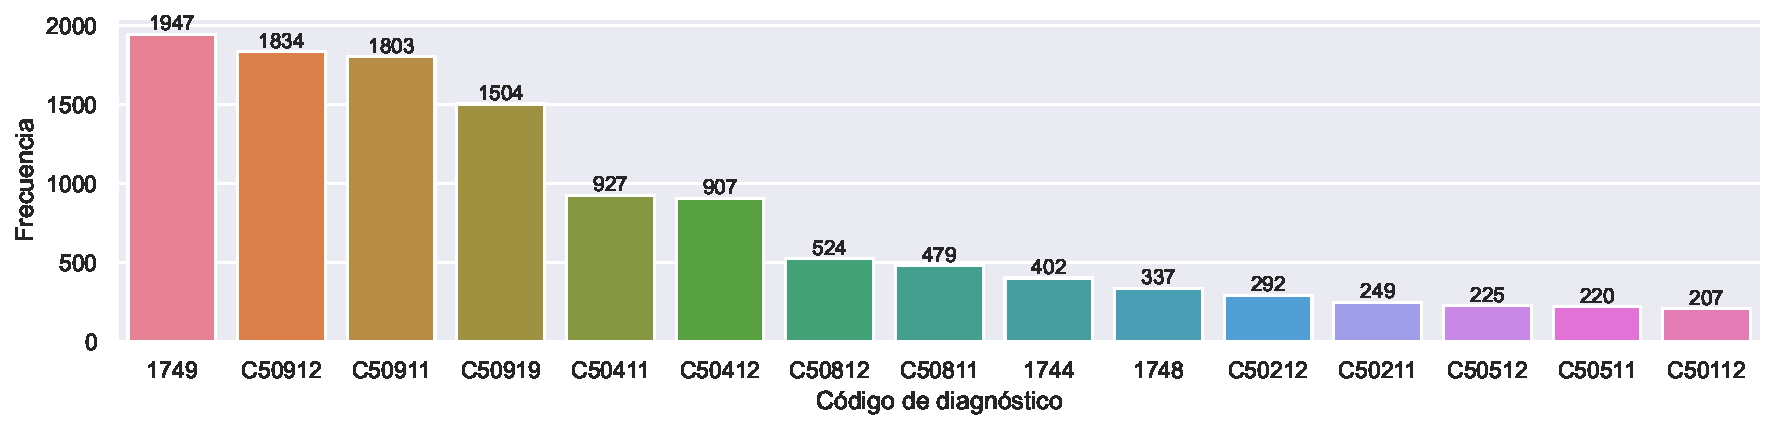
\includegraphics[width=0.9\linewidth]{figs/chapter3/categorical/bcdistribution}
					\caption{General}\label{fig:ch3bcdist}
				\end{center}
			\end{subfigure} 
			\begin{subfigure}{\linewidth}
				\begin{center}
					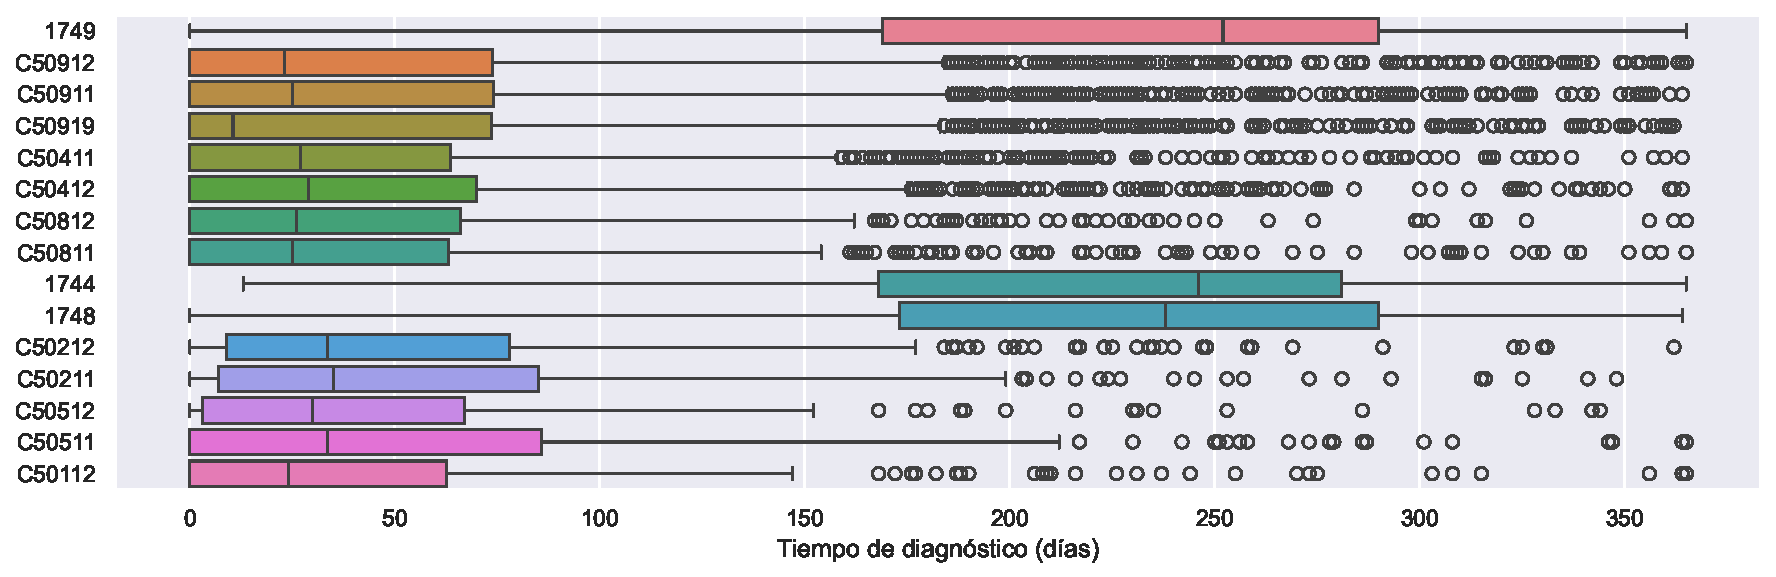
\includegraphics[width=0.9\linewidth]{figs/chapter3/categorical/bcperiod}
					\caption{Respecto al tiempo de diagnóstico}\label{fig:ch3bcperiod}
				\end{center}
			\end{subfigure} 
		\end{center}
		\captionsetup{aboveskip=-5pt, belowskip=-15pt, justification=centering}
		\caption{Distribución de los 15 valores más frecuentes del código de diagnóstico de cáncer de mama}
		\label{fig:ch3bc}
	\end{figure}
	
	En la \textbf{Figura \ref{fig:ch3bcdist}} se estudia la distribución general, y como se puede observar, \textbf{existen dos tipos de codificaciones} - las codificaciones que empiezan por la letra \textbf{C} (ICD10, más moderno) y las que empiezan por un número (ICD9). Además, se puede ver que la mayoría de diagnósticos se encuentran agrupados en cuatro códigos - con la frecuencia del resto de atributos bajando rápidamente hasta llegar a los diagnósticos con una o dos instancias no representados. Estos diagnósticos, si se comprueba su código descriptivo, hacen referencia a \textbf{cánceres en sitios sin especificar} - es decir, los códigos más genéricos y por tanto aplicables a un mayor número de casos.

	En la \textbf{Figura \ref{fig:ch3bcperiod}} se puede apreciar una diferencia clara en tiempos de diagnóstico dependiendo de la \textbf{codificación utilizada}, con los diagnósticos con codificación de tipo \textbf{ICD9} teniendo un tiempo de diagnóstico promedio notablemente superior. Si bien no hay una explicación clara para ésto, puede deberse a que hagan referencia a casos más antiguos - y, por tanto, casos con menor conocimiento y recursos.
	
	Por esto, resulta evidente que el código de diagnóstico de cáncer de mama ofrece información discriminatoria muy relevante de cara a ser utilizada en el modelo posterior.
	
	\item \textbf{Código de diagnóstico de cáncer metastásico:}
	
	A diferencia del código de diagnóstico para cáncer de mama, para el \textbf{diagnóstico de cáncer metastásico} solo se tiene un atributo. 
	
	Ahora bien, se sigue teniendo el mismo problema de dimensionalidad: el conjunto de datos contiene \textbf{43 valores únicos} para este atributo, sin garantía de que sea un conjunto \textbf{exhaustivo}. Por esto, se realizará el estudio sobre los \textbf{15 códigos más frecuentes}.
	
	\begin{figure}[h]
		\begin{center}
			\begin{subfigure}{\linewidth}
				\begin{center}
					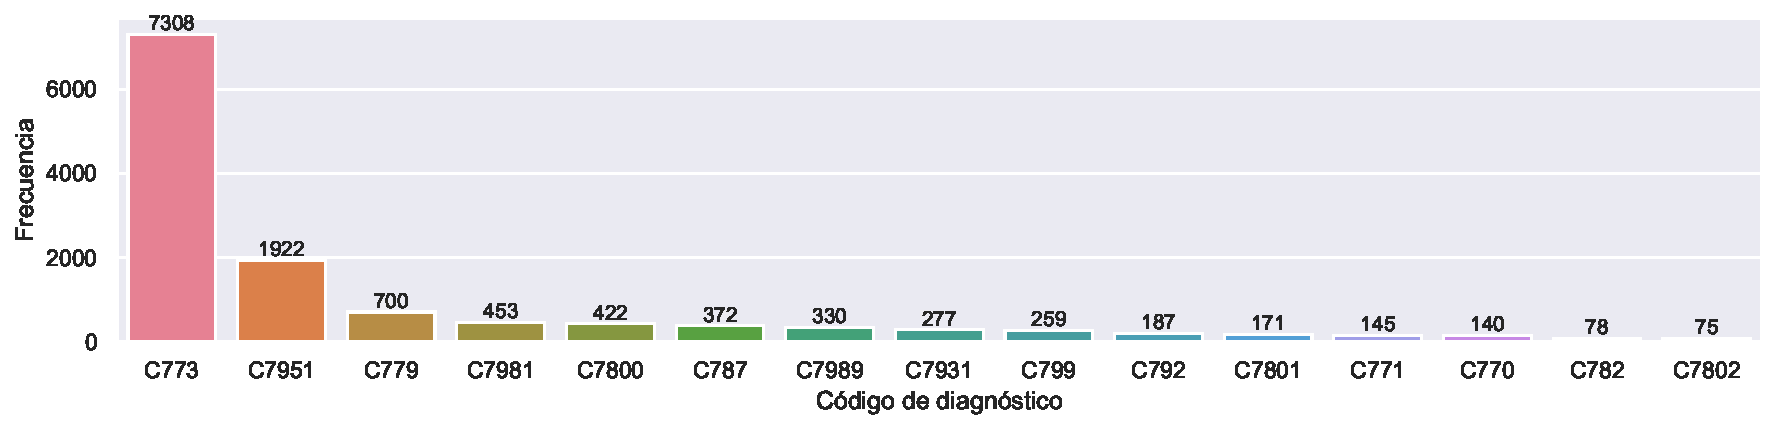
\includegraphics[width=0.9\linewidth]{figs/chapter3/categorical/mcdistribution}
					\caption{General}\label{fig:ch3mcdist}
				\end{center}
			\end{subfigure} 
			\begin{subfigure}{\linewidth}
				\begin{center}
					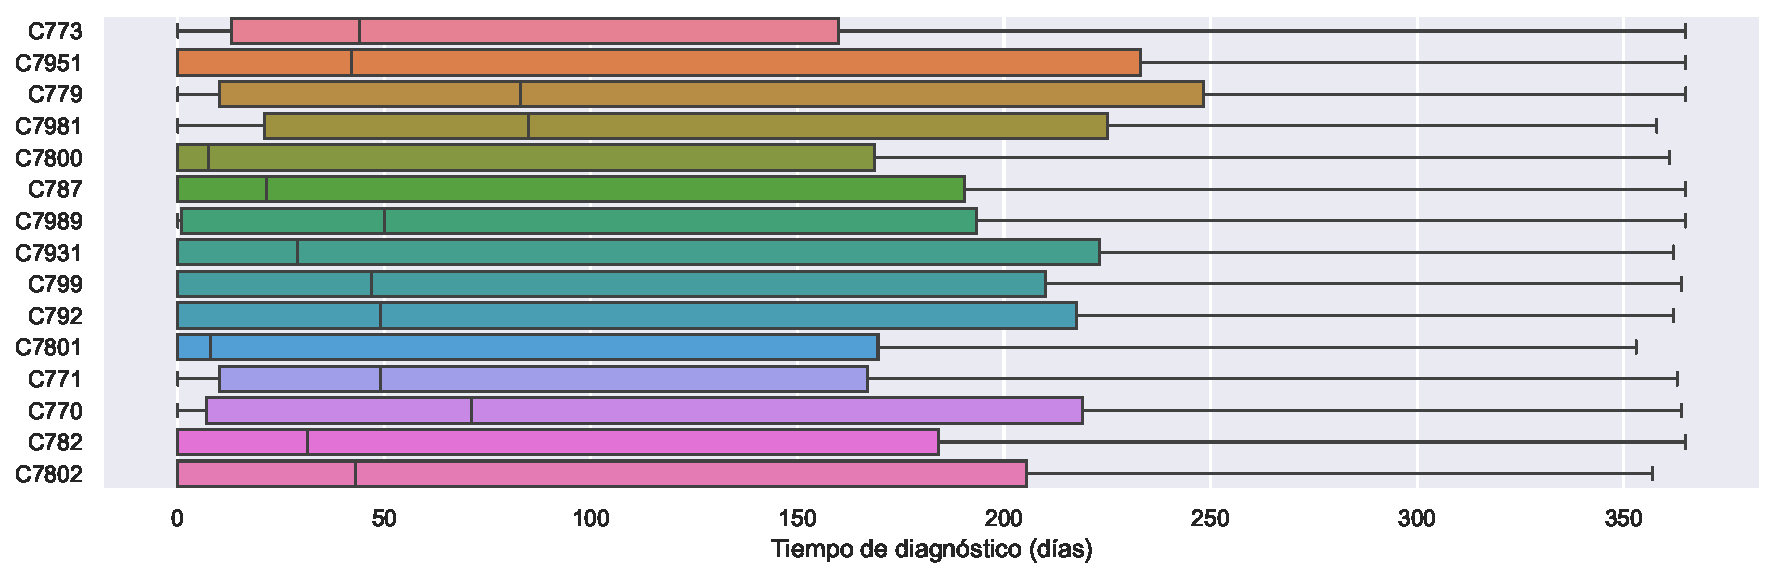
\includegraphics[width=0.9\linewidth]{figs/chapter3/categorical/mcperiod}
					\caption{Respecto al tiempo de diagnóstico}\label{fig:ch3mcperiod}
				\end{center}
			\end{subfigure} 
		\end{center}
		\captionsetup{aboveskip=-5pt, belowskip=-15pt, justification=centering}
		\caption{Distribución de los 15 valores más frecuentes del código de diagnóstico de cáncer de mama}
		\label{fig:ch3mc}
	\end{figure}
	
	Como se observa en la \textbf{Figura \ref{fig:ch3mcdist}} y a diferencia del diagnóstico de cáncer de mama, en este caso \textbf{la mayoría de diagnósticos se concentran alrededor de un único diagnóstico} - $C773$, metástasis en nodos linfáticos auxiliares y de las extremidades superiores -, con el resto de diagnósticos reduciendo su frecuencia rápidamente.
	
	Respecto a la relación con el tiempo de diagnóstico, en la \textbf{Figura \ref{fig:ch3mcperiod}} se puede ver que, si bien no hay una diferencia tan pronunciada como en el caso del código de diagnóstico de cáncer de mama, \textbf{el tipo de metástasis diagnosticado parece tener influencia sobre el tiempo necesario para su diagnóstico}. Ahora bien, si se estudia la localización de la metástasis de cada código estudiado \textbf{no se observa correlación entre la localización y el tiempo de diagnóstico}.
	
	Por esto, se puede considerar al \textbf{código de diagnóstico del cáncer metastásico} otra variable de gran interés para los modelos desarrollados posteriormente - pudiendo ofrecer una gran capacidad discriminatoria.
	
	\item \textbf{Tipo de tratamiento:}
	
	Como se mencionó durante el estudio de los valores perdidos, \textbf{solo se tienen 11 valores} para este atributo - de \textbf{13173} instancias totales. Por tanto, no tiene ningún sentido estudiar este atributo, al no contener suficiente información para ser significativo.
\end{itemize}

\subsubsection{Datos geográficos - estado de residencia y ubicación geográfica}

El estudio de la información geográfica del conjunto de datos es de especial importancia al ser uno de los objetivos planteados por el problema a resolver. Además, toda la información socio-económica y climática del conjunto de datos está \textbf{asociada al código zip de los pacientes} - por lo que estos atributos codifican de forma innata todos estos factores de sesgo.

Ahora bien, la información se encuentra representada en el conjunto de datos a través de \textbf{4 atributos jerárquicos}, donde cada atributo inferior describe con más granularidad el atributo superior. Al codificar la misma información, es de interés seleccionar \textbf{un único atributo} sobre el que realizar el estudio.

\begin{table}[h]
	\centering
	\resizebox{\textwidth}{!}{%
		\begin{tabular}{@{}rlll@{}}
			\toprule
			\multicolumn{1}{c}{}                                    & \multicolumn{1}{c}{}                                           & \multicolumn{2}{c}{\textbf{p-valores (Tests de hipótesis)}}                                       \\ \cmidrule(l){3-4} 
			\multicolumn{1}{c}{\multirow{-2}{*}{\textbf{Atributo}}} & \multicolumn{1}{c}{\multirow{-2}{*}{\textbf{Valores totales}}} & \textbf{Paramétrico (ANOVA)}                    & \textbf{No paramétrico (Kruskal)}               \\ \midrule
			\textbf{Región}                                         & 4                                                              & $2,80 \times 10^{-3}$                           & $1,93 \times 10^{-6}$                           \\
			\rowcolor[HTML]{EFEFEF} 
			\textbf{División}                                       & 8                                                              & $6,13 \times 10^{-3}$                           & $1,68 \times 10^{-5}$                           \\
			\textbf{Estado}                                         & 44                                                             & $5.86 \times 10^{-10}$                          & $1.06 \times 10^{-16}$                          \\
			\rowcolor[HTML]{EFEFEF} 
			\textbf{Código zip}                                     & 751                                                            & \multicolumn{1}{c}{\cellcolor[HTML]{EFEFEF}---} & \multicolumn{1}{c}{\cellcolor[HTML]{EFEFEF}---} \\ \bottomrule
		\end{tabular}%
	}
	\captionsetup{belowskip=-15pt}
	\caption{p-valores de los atributos geográficos}
	\label{tab:ch3geographical}
\end{table}

Para realizar la selección se han realizado \textbf{tests de hipótesis} - tanto paramétricos (\textbf{ANOVA}, para estudiar desviaciones en la media) como no paramétricos (\textbf{Kruskal-Wallis}, para estudiar desviaciones en la mediana) - sobre todos los atributos excepto el código zip, debido a su alta dimensionalidad. Los resultados se pueden observar en la \textbf{Tabla \ref{tab:ch3geographical}}, siendo el atributo a seleccionar el \textbf{estado}, al tener el p-valor más bajo - y, por tanto, tener la mayor certeza de que \textbf{su valor influye sobre el promedio del tiempo de diagnóstico}.

\begin{figure}[h]
	\begin{center}
		\begin{subfigure}{0.9\linewidth}
			\begin{center}
				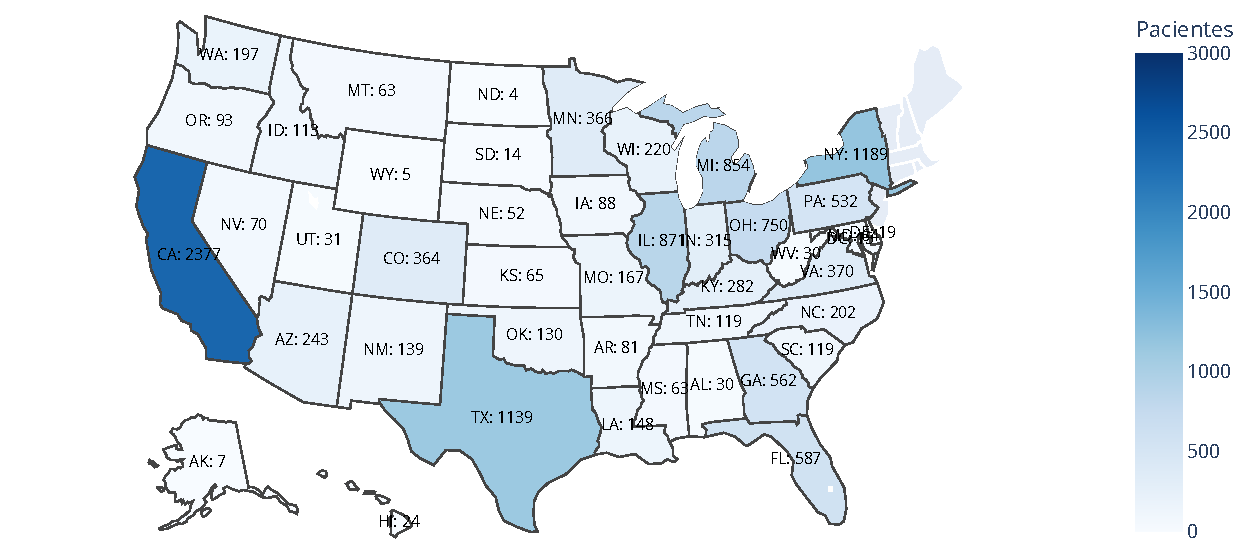
\includegraphics[width=\linewidth]{figs/chapter3/categorical/statedist}
				\caption{Frecuencia}\label{fig:ch3statedist}
			\end{center}
		\end{subfigure} 
		\begin{subfigure}{0.9\linewidth}
			\begin{center}
				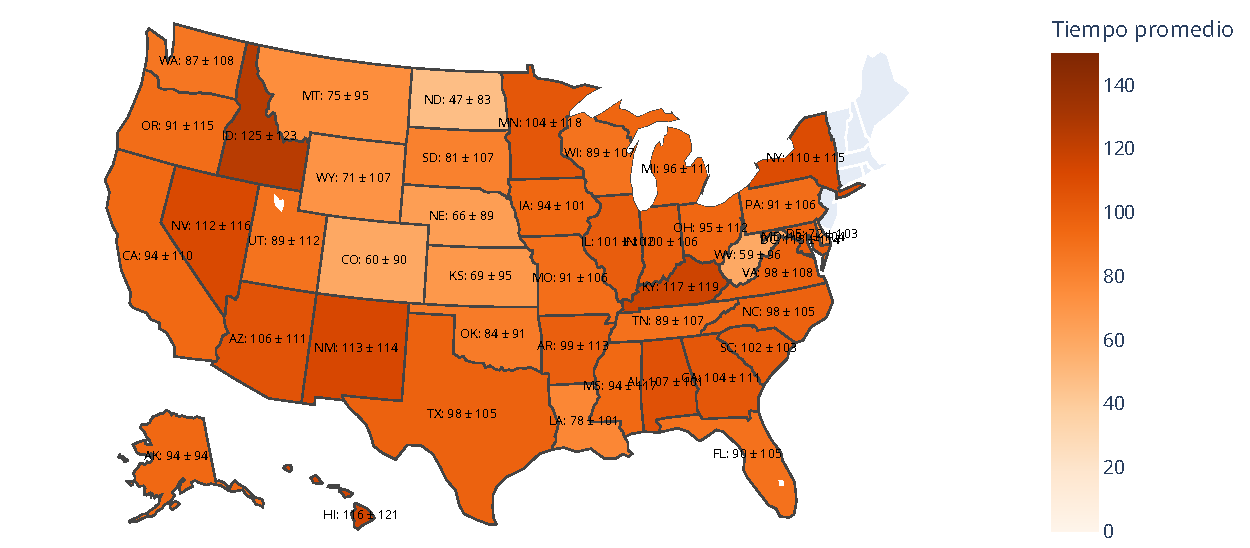
\includegraphics[width=\linewidth]{figs/chapter3/categorical/statemean}
				\caption{Tiempo de diagnóstico promedio}\label{fig:ch3statemean}
			\end{center}
		\end{subfigure} 
	\end{center}
	\captionsetup{aboveskip=-5pt, belowskip=-15pt, justification=centering}
	\caption{Distribución geográfica de los pacientes}
	\label{fig:ch3state}
\end{figure}

En el mapa de la \textbf{Figura \ref{fig:ch3statedist}} se representa la distribución de los pacientes en el mapa de los Estados Unidos, donde se observa que los pacientes están \textbf{agrupados en estados concretos} - en general, los estados de mayor población -, sin haber una correlación geográfica clara en su ubicación. También se observa que \textbf{existen algunos estados sin pacientes} - por lo que, igual que con los códigos de diagnóstico, \textbf{los valores del atributo no son exhaustivos}.

Estudiando el valor promedio del tiempo de diagnóstico, la \textbf{Figura \ref{fig:ch3statemean}} muestra que el \textbf{tiempo de diagnóstico promedio es similar entre todos los estados} - rondando alrededor de los \textbf{80 días}, pero ubicado en el rango de los \textbf{60 a 120 días}. También es llamativo el hecho de que \textbf{la desviación estándar es muy elevada} - en la práctica totalidad de los estados se trabaja con desviaciones estándar de alrededor de \textbf{100 días}.

El test de hipótesis indica que el estado del paciente \textbf{influye de forma significativa sobre el tiempo de diagnóstico}, por lo que es un atributo de interés de cara a la creación posterior de modelos. Ahora bien, el estudio gráfico de la distribución también muestra que existe un \textbf{error sustancial} en dicha diferencia, al haber un rango muy elevado de posibles valores dentro de cada estado.

\subsection{Estudio de atributos numéricos}

Tras el estudio de los atributos categóricos, el siguiente paso es realizar un \textbf{estudio exhaustivo} de los atributos numéricos más significativos. Sin embargo, el elevado número de atributos, con un total de \textbf{138 variables numéricas}, hace imposible el estudio individualizado. Por tanto, el objetivo es seleccionar los \textbf{principales atributos numéricos} - entendiendo como tales los \textbf{atributos con mayor influencia sobre el tiempo de diagnóstico}. 

Una forma de realizar esta selección es mediante el \textbf{coeficiente de correlación de Pearson} - un valor numérico en el rango $[-1, 1]$ indicando la \textbf{relación lineal entre dos atributos}, donde los valores cercanos a los extremos indican una correlación fuerte y un valor cercano a $0$ indica independencia entre los atributos.

\begin{figure}[h]
	\centering
	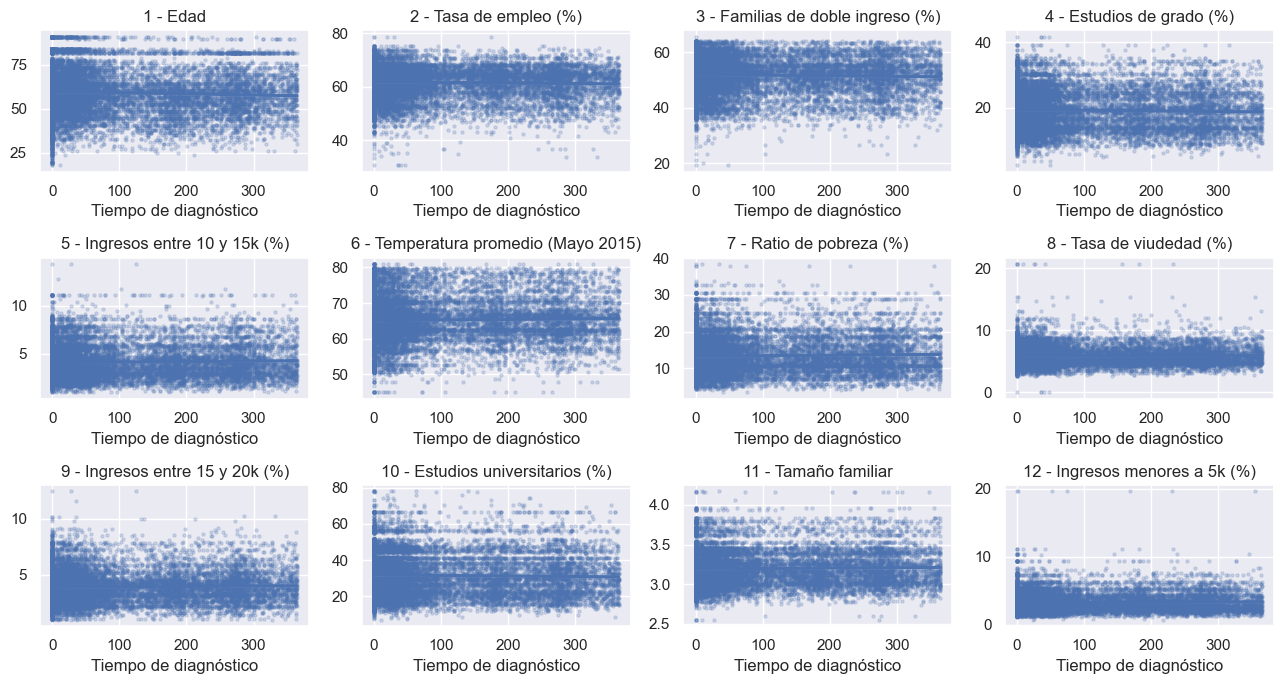
\includegraphics[width=1\linewidth]{figs/chapter3/numerical/correlations.png}
	\captionsetup{belowskip=-15pt, justification=centering}
	\caption{Relación entre valor y tiempo de diagnósticos para los 12 atributos de mayor correlación}
	\label{fig:ch3correlations}
\end{figure}

Ahora bien, como se refleja en la \textbf{Figura \ref{fig:ch3correlations}}, cuando se calcula la correlación entre los \textbf{138 atributos} y el tiempo de diagnóstico se observa claramente que \textbf{los valores de correlación de Pearson son muy bajos} - siendo el valor más alto de $0.055$. Estos valores se traducen en que \textbf{los atributos numéricos no tienen apenas influencia sobre el tiempo de diagnóstico} - y, por tanto, \textbf{pueden ser descartados} en las siguientes etapas del proceso de ciencia de datos.

Al ser la práctica totalidad de atributos socioeconómicos y climáticos de tipo numérico, esto también se traduce en una respuesta al segundo objetivo del problema: identificar que, en contra de lo que se podría esperar, \textbf{los factores socioeconómicos y climáticos no parecen tener influencia sobre el tiempo de diagnóstico} - al menos, para el conjunto de datos proporcionado. 

% 4 - Preprocesamiento de los datos
\chapter{Preparación del conjunto de datos}

En este capítulo se describe el conjunto de transformaciones y técnicas aplicadas sobre el conjunto de datos para transformarlo, para su uso posterior durante las etapas de entrenamiento y experimentación.

En primer lugar se propone un número de \textbf{subconjuntos de atributos} de cara a reducir la dimensionalidad del conjunto de datos. Tras esto, se plantean y describen las \textbf{transformaciones} aplicadas al conjunto de datos previo al entrenamiento para estandarizar los datos y mejorar el rendimiento de los modelos.


\section{Selección de atributos}

Durante el análisis exploratorio se realizó un estudio exhaustivo de los atributos contenidos en el conjunto de datos, en el que se han identificado los siguientes problemas:

\begin{itemize}
	\item \textbf{Alta dimensionalidad:} El conjunto de datos tiene \textbf{150 atributos} en total, donde la mayoría de atributos categóricos tienen \textbf{40 o más valores únicos}. Esto, unido al número de instancias bajo para dicha complejidad, puede significar que el modelo acabaría \textbf{sobreajustándose} al no poder aprender generalizaciones de forma adecuada.
	\item \textbf{Irrelevancia de los atributos:} De los 150 atributos estudiados, \textbf{la amplia mayoría no presentan correlación con la variable objetivo} - por lo que mantenerlos puede implicar una disminución del rendimiento final del modelo y un aumento del tiempo de entrenamiento.
\end{itemize}

Debido a esto, resulta necesario realizar una \textbf{selección de atributos} - proponiendo varios \textbf{subconjuntos de atributos} a evaluar durante la experimentación y selección de modelos, con el objetivo de optimizar el rendimiento del modelo reduciendo la dimensionalidad.

\subsection{Selección manual de atributos}

El primer subconjunto de atributos propuesto se realizar a partir de las observaciones obtenidas a través del análisis exploratorio de datos realizado en el capítulo anterior - estando este formado por las \textbf{variables con mayor significancia para la predicción del tiempo de diagnóstico}, según las gráficas y tests realizados. Tras este estudio, se han seleccionado los siguientes \textbf{5 atributos}:

\begin{itemize}[parsep=1pt, itemsep=1pt, topsep=4pt]
	\item Código de diagnóstico del cáncer de mama.
	\item Código de diagnóstico del cáncer metastásico.
	\item Estado de residencia del paciente.
	\item Raza del paciente.
	\item Tipo de seguro médico del paciente.
\end{itemize}

Como se puede observar, \textbf{todos los atributos seleccionados son categóricos}. Esto se debe a la correlación prácticamente nula entre los atributos numéricos y el tiempo de diagnóstico. Además, se ha optado por representar la información geográfica a través del \textbf{estado de residencia} - al ser el atributo geográfico con menor valor en los tests de hipótesis.

A través de esta selección se ha reducido el conjunto de atributos de \textbf{150 a 5 atributos}, reduciendo sustancialmente la dimensionalidad. Ahora bien, los atributos elegidos siguen siendo complejos debido al gran número de valores posibles, por lo que será necesario un procesamiento posterior para \textbf{agrupar los valores menos frecuentes}.

\subsection{Selección automática de atributos}

El subconjunto de atributos propuesto en la sección anterior está basado en el análisis exploratorio realizado. Ahora bien, al basar la decisión únicamente en tests estadísticos y gráficas - sin evaluar el rendimiento real en modelos, -, existe la posibilidad de que se haya introducido un \textbf{sesgo personal} o que existan otros subconjuntos de atributos que puedan ofrecer un mejor rendimiento.

Con el fin de solucionar estos problemas y de acercar el proceso de selección de atributos al funcionamiento real de los modelos, se proponen \textbf{dos subconjuntos adicionales} obtenidos a través de \textbf{algoritmos de selección automática de variables} \cite{featureselection} - basados en técnicas estadísticas y en entrenamiento de modelos.

\subsubsection{\textit{Filter}: Selección mediante tests estadísticos}

Los \textbf{métodos de filtrado} (también conocidos como \textit{filter}) son algoritmos que evalúan la \textbf{relevancia de cada atributo} a través de tests estadísticos, sin necesidad de entrenar ningún modelo - lo que los hace más ágiles que otros métodos, pero más genéricos e incapaces de encontrar todas las correlaciones entre grupos de atributos \cite{featureselection}.

Para este problema se ha utilizado un \textbf{test estadístico F} - una medida de la \textbf{dependencia lineal} entre atributos -, calculando la correlación entre cada atributo numérico y el tiempo de diagnóstico. A partir de estas puntuaciones, se eligen los \textbf{10 atributos} con mayor dependencia lineal:

\begin{itemize}[parsep=1pt, itemsep=1pt, topsep=4pt]
	\item \textbf{Atributos categóricos (5):} 
	\begin{itemize}[parsep=1pt, itemsep=1pt, topsep=4pt]
		\item \textbf{Código de diagnóstico:} Cáncer de mama y cáncer metastásico.
		\item \textbf{Atributos del paciente:} Tipo de seguro médico, raza y estado de residencia del paciente.
	\end{itemize}
	\item \textbf{Atributos numéricos (5):}
	\begin{itemize}[parsep=1pt, itemsep=1pt, topsep=4pt]
		\item \textbf{Atributos del paciente:} Edad del paciente.
		\item \textbf{Estadísticos socioeconómicos (porcentajes):} Tasa de empleo, habitantes con estudios de grado, familias con dos o mas ingresos y habitantes con estudios universitarios o superiores.
	\end{itemize}
\end{itemize}

El subconjunto de atributos obtenido reafirma la selección manual realizada, al tener ambos conjuntos los \textbf{mismos atributos categóricos} - siendo el \textbf{código de diagnóstico del cáncer de mama} el atributo con mayor relevancia con diferencia. La principal diferencia se encuentra en que se han seleccionado además \textbf{atributos numéricos}, algunos de ellos teniendo incluso mayor relevancia que otros atributos categóricos - como la \textbf{edad del paciente}.

\subsubsection{\textit{Wrapper}: Selección mediante entrenamiento de modelos}

Los \textbf{métodos de envoltura} (también conocidos como \textit{wrapper}) son algoritmos que realizan su selección de atributos a través del \textbf{entrenamiento de un modelo de aprendizaje automático} y la selección de las variables más relevantes en base a los parámetros y pesos aprendidos por el modelo. A diferencia de los métodos de \textit{filter}, el proceso de selección suele ser más lento, pero los resultados suelen ser más fiables al trabajar de forma directa con modelos reales \cite{featureselection}.

Para este problema se ha utilizado un modelo de \textbf{\textit{Random Forests}}, entrenado con los hiperparámetros por defecto de su implementación en \textit{Scikit-Learn} - \textbf{100 árboles} sin profundidad máxima. A partir de este modelo entrenado se extraen los \textbf{10 atributos} con mayor peso sobre el modelo entrenado: 

\begin{itemize}[parsep=1pt, itemsep=1pt, topsep=4pt]
	\item \textbf{Atributos categóricos (4):} 
	\begin{itemize}[parsep=1pt, itemsep=1pt, topsep=4pt]
		\item \textbf{Código de diagnóstico:} Cáncer de mama y cáncer metastásico.
		\item \textbf{Atributos del paciente:} Tipo de seguro médico y raza del paciente.
	\end{itemize}
	\item \textbf{Atributos numéricos (6):}
	\begin{itemize}[parsep=1pt, itemsep=1pt, topsep=4pt]
		\item \textbf{Atributos del paciente:} Edad e índice de masa corporal del paciente.
		\item \textbf{Estadísticos socioeconómicos}: Tiempo de viaje al trabajo promedio, porcentaje de personas de raza nativa, porcentaje de habitantes con estudios STEM, porcentaje de habitantes con edades entre 40 y 49 años.
	\end{itemize}
\end{itemize}

Frente a las selecciones manuales y de filtrado, el \textbf{subconjunto \textit{wrapper} no incluye información geográfica en su selección} - optando, en su lugar, por incluir un mayor número de atributos numéricos tanto médicos como socioeconómicos.

\section{Pre-procesamiento de los datos}

A la par que se propone una selección de atributos para reducir la dimensionalidad del conjunto de datos, resulta también necesario realizar un \textbf{pre-procesamiento} - una serie de transformaciones secuenciales sobre los datos - para reducir la complejidad y paliar posibles problemas como los valores perdidos o la codificación de los atributos categóricos. De esta forma, se busca mejorar el rendimiento de los modelos entrenados.

Ahora bien, los atributos necesitan \textbf{transformaciones distintas} dependiendo del tipo de datos que representen - siendo necesario distinguir entre atributos numéricos y categóricos. Para el trabajo descrito en la memoria, se han propuesto las siguientes transformaciones dependiendo del tipo de datos del atributo:

\begin{itemize}[leftmargin=*, parsep=1pt, itemsep=1pt, topsep=4pt]
	\item \textbf{Atributos categóricos:}
	
	\begin{enumerate}
		\item \textbf{Imputación de valores perdidos:} Como se estudió durante el análisis exploratorio de datos, para la mayoría de atributos categóricos \textbf{resulta de interés tratar los valores perdidos como categorías separadas}, al ser relevante para el estudio que faltasen valores.
		
		Por esto, se opta por reemplazar todos los valores perdidos por un \textbf{valor constante, \textit{"UNKNOWN"}}.
		
		\item \textbf{Codificación:} De forma inherente, la mayoría de modelos propuestos son incapaces de trabajar con atributos categóricos - necesitando transformar estos atributos en algún tipo de codificación numérica.
		
		Para estos casos, lo estándar es utilizar una codificación de tipo \textbf{\textit{One-Hot}} \cite{GVK022791892}: dividiendo el atributo original en \textbf{tantos atributos como valores tiene la variable original}, donde el atributo que se corresponde con el valor de la variable original tiene un valor de $1$ y el resto tiene valores de $0$ - representando de esta manera los valores categóricos en un formato numérico.
		
		Es importante destacar las siguientes particularidades para el problema actual:
		\begin{itemize}
			\item Debido a que los atributos categóricos del conjunto de datos tienen una \textbf{alta dimensionalidad} y \textbf{valores no exhaustivos}, es necesario realizar una \textbf{agrupación de los atributos menos frecuentes y desconocidos} bajo un único atributo $at_{other}$. El umbral para considerar un atributo como poco frecuente será determinado durante el proceso de experimentación y selección de modelos.
			\item La implementación de los modelos de \textbf{\textit{Gradient Boosting}} codifican de forma inherente los atributos categóricos, por lo que no es necesario aplicar este paso para ellos.
		\end{itemize}
		 
	\end{enumerate}
	
	\item \textbf{Atributos numéricos:}
	
	\begin{enumerate}
		\item \textbf{Imputación de valores perdidos:} Debido a la presencia de valores extremos en la mayoría de atributos numéricos, se reemplazan los valores perdidos por el \textbf{valor mediano del atributo al que pertenece} - ofreciendo de esta forma un valor promedio resistente a sesgos y \textit{outliers}.
		\item \textbf{Escalado:} Por lo general, es necesario \textbf{escalar los datos} - transformar los valores de todos los atributos para que se encuentren en el mismo rango - de los atributos numéricos para el funcionamiento adecuado de los modelos.
		
		Para el problema descrito, se intenta evitar los problemas introducidos por los valores extremos utilizando un escalado alrededor de la \textbf{mediana y el rango intercuartil}, donde cada valor se transforma utilizando la fórmula $z(x) = \frac{x - mediana}{IQR}$. 
	\end{enumerate}
\end{itemize}

% 5 - Modelado y experimentación
\chapter{Modelado y experimentación}

\section{Selección de modelos}

\section{Experimentación}

\subsection{Ajuste de hiperparámetros y selección de subconjuntos de atributos}

\subsection{Validación y selección de modelo final}

\section{Análisis de resultados}

\subsection{Rendimiento de los subconjuntos de hiperparámetros}

\subsection{Rendimiento de los modelos entrenados}

\subsection{Rendimiento del modelo final}

% 6 - Aplicación web
\chapter{Aplicación web}

% 8 - Conclusiones
\chapter{Conclusiones}

A lo largo del trabajo realizado y de la memoria, se ha descrito en detalle el \textbf{ciclo de vida de la ciencia de datos} llevado a cabo para resolver el problema planteado: la \textbf{predicción del tiempo de diagnóstico de cáncer metastásico}, en base a datos médicos, geográficos, socioeconómicos y climáticos.

El primer paso ha sido un \textbf{análisis exploratorio de datos}, para conocer y entender mejor el comportamiento del conjunto de datos - lo que ha permitido realizar un \textbf{preprocesamiento} posterior en el que se han seleccionando atributos y transformando los datos para su uso durante el \textbf{modelado}, donde se han planteado una serie de posibles modelos para solucionar el problema. 

El mejor de dichos modelos ha sido seleccionado a través de una \textbf{evaluación} de su rendimiento en comparación con el resto de modelos y con los ganadores de la competición. Finalmente, este modelo se ha dejado disponible a los usuarios finales a través del \textbf{despliegue} de una aplicación web.

Tras el trabajo realizado, se puede afirmar que el \textbf{primer objetivo} - la creación de un modelo de regresión capaz de predecir el tiempo de diagnóstico - se ha \textbf{cumplido con éxito} dentro de las posibilidades:
\begin{itemize}
	\item El modelo entrenado \textbf{presenta un error elevado} - alrededor de \textbf{82 días} en promedio -, si bien dicho error se encuentra cercano al error de los modelos ganadores de la competición.
	\item El funcionamiento del modelo es \textbf{ágil} - en el orden de los segundos para el entrenamiento y de los milisegundos para la predicción -, lo que lo hace \textbf{utilizable en tiempo real}.
	\item La \textbf{aplicación web} permite el uso simple del modelo por parte de los usuarios finales.
\end{itemize}

Respecto al \textbf{segundo objetivo} - el estudio de la influencia de factores geográficos, socioeconómicos y climáticos -, se han extraído las siguientes conclusiones:
\begin{itemize}
	\item El análisis exploratorio de datos indica que \textbf{solo la información médica es relevante para la predicción del tiempo} - los atributos socioeconómicos y climáticos \textbf{no presentan correlación clara con el tiempo de diagnóstico}, y el único atributo geográfico con cierta relevancia es el \textbf{estado de residencia del paciente}.
	\item Pese a esto, \textbf{el modelo final seleccionado incluye información socioeconómica} - en la forma de información estadística sobre los estudios universitarios y los ingresos de las familias. Ahora bien, en la práctica \textbf{dichas variables no tienen apenas influencia sobre el tiempo predicho}.
\end{itemize}

Actualmente, el trabajo completo se encuentra disponible en un repositorio público de \textit{Github} (\url{https://github.com/MoonDollLuna/cidaen_m5_thesis}) bajo licencia \textit{MIT}, incluyendo tanto la memoria como el \textbf{código Python} utilizado para realizar todos los pasos del proceso de ciencia de datos.

Además, como ya se ha comentado en el Capítulo 6, la aplicación web a través de la que se ha desplegado el modelo se encuentra disponible en el enlace \url{https://cidaen-m5-thesis-lunajimenezfernandez.streamlit.app/}.


\section{Trabajo futuro}

El trabajo propuesto fue concebido como parte de una competición ya clausurada, por lo que no tiene sentido continuarlo directamente. Ahora bien, sí es posible plantear una serie de \textbf{ampliaciones al proceso realizado}, de cara a futuros trabajos de ciencia de datos:
\begin{itemize}[parsep=2pt, itemsep=2pt, topsep=4pt]
	\item \textbf{Ampliación del número de modelos:} Aun utilizando los modelos más comunes para problemas de ciencia de datos estructurados, es posible utilizar otra serie de modelos más complejos - como pueden ser las \textbf{redes neuronales} o los \textbf{\textit{stacks}} de \textit{ensembles}.
	\item \textbf{Creación de atributos:} Si bien se ha realizado un pre-procesamiento de los datos, podría haber resultado de interés añadir \textbf{atributos sintéticos} para ampliar la información útil contenida en el conjunto de datos.
	\item \textbf{Modelo disponible a través de cliente - servidor:} Actualmente, el modelo se encuentra embebido en la aplicación web - algo factible debido al tamaño ligero del modelo entrenado, pero que se haría imposible para modelos más complejos o páginas web más concurridas.
	
	Para solucionar ésto, sería razonable crear una \textbf{API (Application Web Interface)} a través de la cual se llamaría al modelo, para hospedarlo en un servidor separado independiente al funcionamiento de la propia aplicación.
\end{itemize}




% -------------------------------
% Bibliografía
% -------------------------------
\printbibliography
\addcontentsline{toc}{chapter}{Referencia bibliográfica} % Añade a la tabla de contenidos

% -------------------------------
% Apéndices
% -------------------------------

\cleardoublepage
\thispagestyle{empty}

\appendix
\chapter{Contenidos del repositorio}

El repositorio en el que se almacena el trabajo realizado y la memoria contiene los siguientes recursos principales:

\begin{itemize}[leftmargin=*]
	\item \textbf{WiDS Datathon 2024 C2 - Part 1 (EDA).ipynb:} Una libreta de \textit{Jupyter} en la que se incluye el proceso de \textbf{exploración de datos}.
	\item \textbf{WiDS Datathon 2024 C2 - Part 2 (Regression Models).ipynb:} Una libreta de \textit{Jupyter} en la que se incluyen los procesos de \textbf{pre-procesamiento}, \textbf{modelado} y \textbf{evaluación} del proceso de ciencia de datos.
	\item \textbf{\textbackslash streamlit:} Una carpeta en la que se contiene todos los ficheros de código \textbf{Python} para el \textbf{despliegue} de la aplicación web a través de la que se hace disponible el modelo.
	\begin{itemize}
		\item Debido al funcionamiento de \textit{Streamlit} a la hora de desplegarse, la mayoría de recursos se encuentran duplicados en la raíz del repositorio.
	\end{itemize}
	\item  \textbf{\textbackslash thesis:} Una carpeta en la que se incluyen todos los ficheros de \textbf{LaTeX} necesarios para la compilación de la memoria.
		
		
\end{itemize}

Además, el repositorio contiene las siguientes carpetas con información adicional utilizada durante el trabajo:

\begin{itemize}[leftmargin=*]
	\item \textbf{\textbackslash data:} Una carpeta con los conjuntos de datos de la competición.
	\item \textbf{\textbackslash models:} Una carpeta con todos los modelos entrenados, tanto los 16 modelos ajustados como el modelo final seleccionado.
	\item \textbf{\textbackslash results:} Una carpeta con todos los resultados de la experimentación, tanto las estadísticas como los hiperparámetros, en formato \textit{CSV}.
\end{itemize}


\end{document}